
\documentclass[11pt,a4paper]{report}		                                   

\usepackage{graphicx}
\usepackage{a4}
\usepackage[english, ngerman]{babel}
%That Headings have Kapitälchen:
\usepackage[T1]{fontenc}

\usepackage{xcolor}

%%%%%%%%%BIBLIOGRAPHY + PICTURES IN TABLE OF CONTENTS
\usepackage[nottoc]{tocbibind}
\usepackage{breakcites}



%%%%%%%%%%%%%%%%%%%%%%%%%%%%%ABKÜRZUNGEN
\usepackage{nomencl}
\let\abbrev\nomenclature
\renewcommand{\nomname}{List of Abbreviations}
\setlength{\nomlabelwidth}{.25\hsize}
\renewcommand{\nomlabel}[1]{#1 \dotfill}
\setlength{\nomitemsep}{-\parsep}
\makenomenclature 
\newcommand{\Abkuerzung}{
    \printnomenclature
    \newpage
}

%%%%%%%%%%%%%%%%%%%%%%%%%%%%%Links
\usepackage{hyperref}
\usepackage{url}
%%%%%%%%%%%%%%%%%%%%%%%%%%%%%Listings
\usepackage{listings} 

\lstdefinestyle{XQuery}{
	language=XQuery,
	float=h,
}

\xdefinecolor{listing-blue}{rgb}{33,43,63}
%\xdefinecolor{listing-green}{rgb}{00A000}
%\xdefinecolor{listing-red}{rgb}{D00000}
%\xdefinecolor{listing-cyan}{rgb}{00A0A0}
%\xdefinecolor{listing-purple}{rgb}{AE26AE}

%%%%%%%%%%%%%%%%%%%%%%%%%%%%XQUERY LANGUAGE
\lstdefinelanguage{XQuery}{
	keywordsprefix=\$,
	keywords={lalalalala},
	morekeywords=[2]{for,let,where,order by,return,ascending,descending,:=,mod,empty in,window,group,toi,fn:data },
%	morekeywords={ancestor,ancestor-or-self,and,as,ascending,at,attribute,base-uri,boundary-space,by,case,cast,castable,
%		child,collation,comment,construction,copy-namespaces,declare,descendant,descendant-or-self,descending,
%		div,document,document-node,element,else,empty,empty-sequence,encoding,eq,every,except,external,following,
%		following-sibling,for,function,ge,greatest,gt,idiv,if,import,in,inherit,instance,intersect,item,lax,le,
%		least,let,lt,mod,module,namespace,ne,node,no-inherit,no-preserve,option,or,order,ordered,ordering,
%		preceding,preceding-sibling,preserve,processing-instruction,return,satisfies,schema,schema-attribute,schema-element,
%		self,some,stable,strict,strip,text,then,treat,typeswitch,union,unordered,validate,variable,version,where,xquery},
	% removed from the list of keywords: parent,is,of,to,default
%	otherkeywords={-,;,::,:=,!=,?,?>,/,//,/>,.,..,(\#,[,],]]>,\{,\},@,\$,*,\#),+,<,<!--,<![CDATA[,<?,</,<<,<=,=,>,-->,>=,>>,|},
%	sensitive,
%	morecomment=[s]{(:}{:)},
	string=[b]",
	morestring=[s]{'}{'},
	morestring=[s]{"`}{"'},
%	morestring=[b]",
%	morestring=[b]',
}

\lstset{
   language=XQuery,
   basicstyle=\footnotesize,
%   backgroundcolor=\color{yellow},
   keywordstyle=\color{yellow},
   keywordstyle=[1]\color{green},
   keywordstyle=[2]\color{blue}, 
   keywordsprefix=\$,
   identifierstyle=,
   commentstyle=\color{green!50!black!100},
   stringstyle=\color{red!100},
   breaklines=true,
   numbers=left,
   tabsize=2,
   numberstyle=\footnotesize,
   frame=single
}

%%%%%%%%%%%%%%%%%%%%%%%%%%%%GNUPLOT
\usepackage{gnuplottex}   
%\usepackage{epstopdf}

\usepackage{amsmath}

%%%%%%%%%%%%%%%%%%%%%%%%%%%QUERTABELLEN
\usepackage{rotating} 

%%%%%%%%%%%%%%%%%%%%%%%%%%%TABELLEN
\usepackage{multirow}

%%%%%%%%%%%%%%%%%%%%%%%%%%%SCHUSTERJUNGEN UND HURENKINDER
\clubpenalty10000
\widowpenalty10000
\displaywidowpenalty=10000

%%%%%%%%%%%%%%%%%%%%%%%%%%%KEIN Ba sex
\selectlanguage{english}
\hyphenation{BaseX}

%%%%%%%%%%%%%%%%%%%%%%%%%%%APPENDIX
\usepackage[toc,page]{appendix}



\newcommand{\thema}{Migrating the XML database \textsc{BaseX} to the Android platform and analyzing the result}
\newcommand{\schlagworte}{\textsc{BaseX}, XML, Database, Android, Performance, SQLite3}
\newcommand{\zusammenfassung}{
The present thesis outlines the migration of the XML database \textsc{BaseX} to the Android platform.
\textsc{BaseX} is available for desktop platforms, therefore it is outlined how Android and those platforms are differ.
All necessary steps to build \textsc{BaseX} on Android are described and the process of creating an Android library which offers all needed \textsc{BaseX} functionalities is shown.
After having created the working Android library of \textsc{BaseX}, the performance of the database has been analyzed and improved.
For this purpose, different benchmarks on various devices have been used to identify the bottlenecks of the mobile \textsc{BaseX} version.
After identifying these problems, it is shown which of them are depending on a specific platform constraint and which can be improved by changing the software.
The performance differences between \textsc{BaseX} and the default Android database SQLite3 are also illustrated and which of these should be prefered for a specific domain.

}
\newcommand{\ausgabedatum}{28.09.2013}
\newcommand{\abgabedatum}{28.03.2014}
\newcommand{\autor}{Stephan Hagios}
\newcommand{\autorStrasse}{Zasiusstra\ss e 17}
\newcommand{\autorPLZ}{78462}
\newcommand{\autorOrt}{ Konstanz}
\newcommand{\autorGeburtsort}{Freiburg, im Breisgau}
\newcommand{\autorGeburtsdatum}{03.07.1985 }
\newcommand{\prueferA}{Prof. Dr. Oliver Eck}
\newcommand{\prueferB}{Dr. Christian Gr\"un}
\newcommand{\prueferC}{Dr. Alexander Holupirek}
\newcommand{\firma}{\textsc{BaseX} GmbH}
\newcommand{\studiengang}{Master of Science Informatik}


\begin{document}


\begin{titlepage}

\vspace*{-3.5cm}

\begin{flushleft}
\hspace*{-1cm} 
\includegraphics[width=15.7cm]{htwg-logo.pdf}
\end{flushleft}

\vspace{2.5cm}

\begin{center}
	\huge{
		\textbf{\thema} \\[5cm]
	}
	\Large{
		\textbf{\autor}} \\[6.5cm]
	\large{
		\textbf{Konstanz, \abgabedatum} \\[2.3cm]
	}
	
	\Huge{
		\textbf{{\sf MASTERARBEIT}}
	}
\end{center}

\end{titlepage}

\thispagestyle{empty}
{
\setlength{\parskip}{0.5cm}
        \begin{center}
        \textbf{\huge MASTERARBEIT}

        \textbf{zur Erlangung des akademischen Grades}

        \textbf{\Large Master of Science (M. Sc.)}

        \textbf{an der}

        \textsf{\huge Hochschule Konstanz}\\
        {\small Technik, Wirtschaft und Gestaltung}

        \textsf{\Large Fakult"at Informatik} \\
        Studiengang \studiengang
        \end{center}
}
\begin{center}

\vspace*{2cm}

\begin{tabular}{p{3cm}p{10cm}}
Thema: & \textbf{\large \thema} \\[15ex]
Masterkandidat: & \autor, \autorStrasse, \autorPLZ  \autorOrt \\[15ex]
1. Pr"ufer: & \prueferA \\
2. Pr"ufer: & \prueferB \\[25ex]
Ausgabedatum: & \ausgabedatum \\
Abgabedatum: & \abgabedatum \\
\end{tabular}
\end{center}

\begin{center}
{\Large \textbf{Zusammenfassung (Abstract)}}
\end{center}

\bigskip

\begin{center}
	\begin{tabular}{p{2.8cm}p{10cm}}
		Thema: & \thema \\
		 & \\
		Masterkandidat: & \autor \\
		 & \\
		Firma: & \firma \\
		 & \\
		Betreuer: & \prueferA  \\[.5ex]
		 &  \prueferB \\
		 & \\
		Abgabedatum: & \abgabedatum \\
		 & \\
		Schlagworte: & \schlagworte \\
		 & \\
	\end{tabular}
\end{center}

\bigskip

\noindent
\zusammenfassung
\chapter*{Ehrenw"ortliche Erkl"arung}
\addcontentsline{toc}{chapter}{Ehrenw"ortliche Erkl"arung}

Hiermit erkl"are ich
\textit{\autor, geboren am \autorGeburtsdatum in \autorGeburtsort}, dass ich\\

\begin{tabular}{lp{12cm}}
(1) & meine Masterarbeit mit dem Titel \\[1em]
& \textbf{\thema} \\[1em]
& bei der \firma\ unter Anleitung von \prueferA\ selbst"andig und ohne fremde Hilfe angefertigt und keine anderen als die angef"uhrten Hilfen benutzt habe;\\[1em]
(2) & die "Ubernahme w"ortlicher Zitate, von Tabellen, Zeichnungen, Bildern und
Programmen aus der Literatur oder anderen Quellen (Internet) sowie die Verwendung
der Gedanken anderer Autoren an den entsprechenden Stellen innerhalb der Arbeit
gekennzeichnet habe.\\
\end{tabular}

\vspace*{1cm}

\noindent
Ich bin mir bewusst, dass eine falsche Erkl"arung rechtliche Folgen haben wird.\\

\vspace*{3cm}

\noindent
Konstanz, \abgabedatum \hfill \begin{tabular}{c} \\ \\ \rule{5cm}{1pt} \\ (Unterschrift)\end{tabular}


\selectlanguage{english}
\tableofcontents
\listoffigures
\renewcommand{\lstlistlistingname}{Listings}
\lstlistoflistings
\addcontentsline{toc}{chapter}{Listings}
\newpage
\addcontentsline{toc}{chapter}{\nomname}
\Abkuerzung

%%% Chapters
\chapter{Introduction}
\label{cha:introduction}
In the last five years, since the release of the first Android phone in October 2008, a lot of progress in the field of mobile devices has been made.
Looking at the market share in the beginning of 2009 shows an amount of 2.8\% sold Android phones~\cite{gandhewar2010google}.
Compared to this, five years later, more than 80\% of the sold smart phones are using Android as their operating system.
This is only one aspect that illustrates the triumphal course Android has made the last few years.
In addition to this the number of available applications for Android phones increase also and has reached more than a million in the third quarter of 2013.
Google offers with its android Play Store the possibility for every developer to easy distribute his application, and offers the possibility to reach millions of customers world wide.


According to bla bla mobile everywhere. Android, And data everywhere, so it's clear to combine database and android.. bla bla
only one solution for android, bla bla, sqlite3
no XML database for android, but needed because of bla bla
then 

\section{Motivation}
\label{sec:introduction:motivation}
Besides the fact that Android is becoming more popular with every sold smartphone or tablet PC, it is also getting more successful in other fields.
For example there exists research about its abilities to be an embedded systems operating system. ~\cite{lee2010evaluating}~\cite{maia2010evaluating}
As well as an operating system for board computers in newer cars, to provide navigation, entertainment and status information.~\cite{macario2009vehicle}
Looking at its triumphal procession in the last three years, it can be said that it will play an important role in the future as an operating system which can be used in a big variety.\\
The same applies for the storage format XML, which has been become more important in the last years, since its release in 1998.



It is obvious that sooner or later an implementation of a native XML database for Android is made.
This thesis outlines a first approach to offer developers the ability to use an XML database and an XQuery processor for their Android applications.

\section{Overview}
\label{sec:overview}
The present thesis outlines the migration of the native XML database \textsc{BaseX} to the Android operating system.
Therefore, first an outline is given, about the database, the Android operating system and if there exist related work to the topic.
This section also underlines that there is no native XML database available for Android, which emphasizes the purpose of the present thesis.
In Chapter~\ref{sec:migration:porting-basex-to-android} the source and target platforms of \textsc{BaseX} has been analyzed as well as the internal dependencies which \textsc{BaseX} is using.
After this the database has been migrated to the Android platform, a library has been created which provides the usual \textsc{BaseX} operations.
At the end of the chapter the problems and issues, as well as their solutions, during the migration have been illustrated.
In the next chapter the ported version of \textsc{BaseX} has been analyzed with different techniques and the bottlenecks have been identified.
The Android library has been optimized by improving the found bottlenecks.
In the last chapter a summery is given as well as a conclusion and proposals for future work which could pick up where the thesis ends.



\chapter{Overview}
\label{cha:overview}
In the following chapter an overview of the used components is given.
It also outlines the used technologies of the present thesis.
%It also describes the actual state of the art of XML database as well as on overview of available mobile operating system.
First an introduction in the native XML database \textsc{BaseX} is given and then the mobile operating system Android is introduced.
At the end of the chapter it is outlined if there is any related work available and how this is important or impacting the present thesis.


%\section{Overview of native XML Databases}
%\label{sec:overview:overview-of-native-xml-databases}
%Databases are used for storing bla blub, there are several types of database, they differ in their way to store and process data.
%
%\section{Overview of Mobile Operating Systems}
%\label{sec:overview:overview-of-mobile-operating-systems}
%MAYBE

\section{Introduction into \textsc{BaseX}}
\label{sec:overview:introduction-into-basex}
\textsc{BaseX} is an XML database that also offers the possibility to process XPath/XQuery.

\section{Overview of Android}
\label{sec:overview:overview-of-android}
Android is an operating system developed by Google and first released in October 2008.~\cite{developers2011android}
It is mostly open source and available in version 4.4.

\section{Related Work}
\label{sec:overview:related-work}
Android offers a SQLite database which can be accessed from the application by using Java libraries.
SQLite is a relational database system specially designed for embedded devices with a low requirement of resources.
It provides beneath all relevant SQL commands also other mechanisms like views or triggers.~\cite{owens2006definitive}
With its low hardware requirement and its a perfect relative database for the Android operating system.
But it is also the only database available on Android.
According to \cite{lamb2010berkleydb} there is an Android implementation of the BerkleyDB database, but it appears not very common, because this is the only reference found to this topic.
Unlike SQLite is BerkleyDB not a relational database, but it is also aims to be deployed on embedded devices.
Another difference between both databases is that SQLite is implemented in C and the Android version of BerkleyDB uses Java as programming language.
Although not showing any test data or benchmark results, \cite{lamb2010berkleydb} claims this the reason that the BerkleyDB is faster than SQLite on a Android device.
Despite this statement those databases are the only available ones for Android and with the BerkleyDB not natively covered by Android, there is no real alternative to SQLite if an Android application is in need of a database.\\
XML BLA BLUB



Zürich xml database and the try to make it available on android.
libxml Linux stuff thing, I compiled it. runs on Android.

\chapter{Porting \textsc{BaseX} to the Android platform}
\label{sec:migration:porting-basex-to-android}
In the present chapter it is shown how the \textsc{BaseX} database has been migrated to the Android platform.
To achieve this goal the source and target platforms have been analyzed and all requirements have been determined.
The main focus lies on the different software platforms and not the hardware specific aspects, due to the big variety of systems and devices which are able to execute both platforms. 
Therefore the two virtual machines and their execution byte formats have been compared and also the specific Android internal mechanisms have been explored.
In Section~\ref{sec:migration:problems-during-the-migration} it is illustrated which parts of the \textsc{BaseX} version have been changed and in which way to receive a working \textsc{BaseX} Android version.
The next section outlines the creation of a client server architecture using \textsc{BaseX} on the Android operating system.
The last section of the present chapter describes the problems which occurred during the migration of the database to Android.

\section{Analyzing the source and target platforms} 
\label{sec:migration:analysing-the-source-and-target-platform}
This section outlines the two different platforms and their specific properties by analyzing them.
The main part of it concentrates on the software part, because both platforms can be executed on a huge amount of hardware devices.
The term platform is hereby defined as on one side the Java Virtual Machine (JVM) and on the other side the Dalvik Virtual Machine (Dalvik VM, or DVM) in the Android environment.
For a better identification the JVM is marked as the source and the DVM as the target platform.
In later sections the Android operating system is also termed as target platform.
\\
The JVM and the DVM are both virtual machines (VM), but they vary in many different ways.
To clarify the term virtual machine it has to be said that a VM is a simulated computer, which can be a whole system with all parts a normal computer provides and also needs to execute a program.
Or it is an abstraction layer which provides the functionality to execute a program on every system that runs the virtual machine.
Unlike compiled machine code a program for a virtual machine is platform independent, because it does not matter on which operating system it is executed, as long as the virtual machine is available for the specific operating system.
A disadvantage of this is the loss of speed, which is a result of the execution of the virtual machine and not only the program in general.~\cite{craig2006virtual}
\\
For both virtual machines the programming language Java is used, which is being compiled into code that the VMs understand and are able to execute.
Although both platforms are virtual machines they differ in some crucial ways.
One of the main difference is that the JVM is a stack based and the DVM is a register based virtual machine.
Another distinctness of both machines is that the DVM is optimized to be executed on mobile devices, meaning that it is designed to use less memory and having a low CPU usage than the JVM.
Lesser hardware usage implies also lesser battery usage, which is also a factor which should be considered in the field of mobile development.\\
Another difference, which need to be considered, is the host system, which is in the DVM case only Android.
And as opposed to this it could be Windows, Mac OS, or any Linux/Unix derivate as host system running a Java virtual machine. 
This circumstance has to be considered if external sources will be used, like writing or reading a file, which is different in every operating system.


\subsection{Comparison of the two virtual machines}
\label{sec:migration:comparison-of-the-two-virtual-machines}
As mentioned in the chapter before both source and target platforms are using Java as a programming language.
Compared to other general purpose programming languages, for example C++, Java is not being compiled into machine code.
To execute Java code a virtual machine is required, that executes the compiled Java code.
However, as in Section~\ref{sec:migration:analysing-the-source-and-target-platform} explained both platforms have different virtual machines.
They differ in many kinds which the application developer not sees but need to consider.
\\
One of the most important differences is that the JVM is stack and the DVM is a register based virtual machine.
This difference helps the DVM to execute the same code in lesser operations than the JVM.
This means that the DVM need lesser CPU cycles than the JVM, which is an improvement that is necessary because of the lack of CPU and memory resources in mobile devices and the aspect of the battery usage.
This can be demonstrated by comparing the instructions done by adding two integers in both virtual machines.
The stack based virtual machine has to execute four machine instructions, while the register based VM can do the same operation in one instruction.
The reason for this is that the stack based VM needs to pop the two values first before it can add and store them back on the stack.
The instructions are \textit{'pop 1', 'pop 2', 'add 1 2', 'push result'}.\\
Figure~\ref{fig:stack-based-addition} illustrates the instruction steps which need to be performed to execute an addition with a stack based virtual machine.
\begin{figure}[h]
\begin{center}
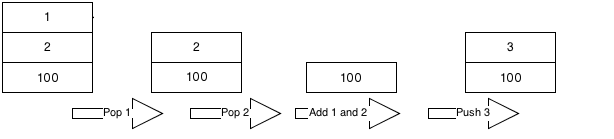
\includegraphics[scale=0.65]{images/stack-based-addition.png} 
\caption{The addition of two integers on a stack based virtual machine.}
\label{fig:stack-based-addition}
\end{center}
\end{figure}
\newpage
Compared to this, the register based virtual machine just needs one machine instruction to complete the same addition of two numbers.
The required instruction is \textit{'ADD R1, R2, R3'}, which can be translated into: add the contents of register 1 and register 2 and store the result in register 3.
Figure~\ref{fig:register-based-addition} illustrates this by showing the add operation of the numbers one and two.
\begin{figure}[h]
\begin{center}
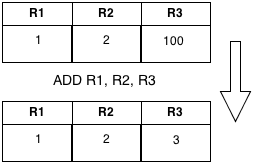
\includegraphics[scale=0.65]{images/register-based-addition.png} 
\caption{The addition of two integers on a register based virtual machine.}
\label{fig:register-based-addition}
\end{center}
\end{figure}

This minimal example shows how the register based virtual machine uses lesser machine instructions compared to the stack based.
The disadvantage in this is that the register based machine has to store the addresses, meaning the corresponding registers, of the operands.
Which is not necessary at a stack based machine, because of the stack pointer that always directs to the actual operand using the Last In First Out (LIFO) principal.
This leads to the result, that stack based code is smaller than the equivalent register based code.
Although the Dalvik VM is a register based virtual machine, the executed byte code is not bigger than the equivalent JVM code.~\cite{shi2008virtual}\\
This is the result of the different formats of the executable virtual machine code, which is optimized in the case of the Davlik virtual machine and is illustrated in Chapter~\ref{sec:comparison-of-the-two-bytecode-formats}.
\\
The code that represents the instructions which are executed on Dalvik VM or the JVM is called bytecode.
To execute this instructions virtual machines having an interpreter which interprets all instructions and performs them.
The difference to normal interpreted languages is, that the JVM or DVM interpreter do not need to check the syntax of the program.
This has been already done by the Java compiler which compiles the Java source code into class files.
Even if it is faster than other interpreted languages, it is still slower than code that is compiled into a machine language and executed directly on the hardware.
This so called machine code is faster because there is no layer between the executions and the hardware, which could slow down the execution.~\cite{aycock2003brief}\\
There is a technique which can improve a virtual machine in performance aspects by adding a Just In Time (JIT) compiler to it.
In general it can be said, that a JIT compiler, used by a virtual machine, compiles heavy used code segments or very expensive calculations into the faster machine code.
There is a great number of different types of JIT compilers and how they work, the two used by the JVM or the DVM are:
\begin{itemize}
\item method-based
\item trace-based
\end{itemize}
The trace-based method works by looking at the most executed code fragments, especially loops, and compiles them into native machine code.\\
The method-based JIT mechanism, in contrast to the trace-based, compiles whole methods, which are often used and expensive in execution time, into native machine code.
Since the release of the Android version 2.2, release name Froyo, the Dalvik VM has received a JIT compiler additionally to the interpreter mechanism.
According to \cite{cheng2010jit} the implemented Dalivk JIT compiler can speed up the execution of intensive operations up to five times.
The Dalvik VM uses the above mentioned mechanism of a trace-based JIT compiler mixed with the usual DVM interpreter.
The given advantage of the trace-based method is that not whole methods are being compiled into machine code.
Instead only the parts which are often executed are being compiled.
This reduces the size of the code which needs to be compiled by the JIT and also omits the not so often executed methods parts like exception handling.
It is needles to compile such parts in machine code to speed them up, because most of the execution time of the program they are not being called.
It should also reduce the compile time for the JIT, because of the selective compilation into machine code.\\
To realize this the Dalvik virtual machine has received an additional thread, which is responsible for the JIT compilation.
Beneath this new thread there is the main thread, that includes the interpreter.
This interpreter interprets the bytecode and records the traces and their occurrence.
If the amount of the occurrence is higher than a predefined number, the trace is being stored into the trace queue.
The new added thread, the JIT thread, compiles the traces from the queue and writes the machine code into the code cache.
The main thread now is doing a lookup if the bytecode that needs to be executed is available in the code cache, at the moment.
If this condition is met, it uses the machine code from the code cache instead interpreting the bytecode.\cite{oh2012evaluation}
Picture~\ref{fig:dvm-threads} illustrates the principle of the two threads in the DVM.\\
\begin{figure}[h]
\begin{center}
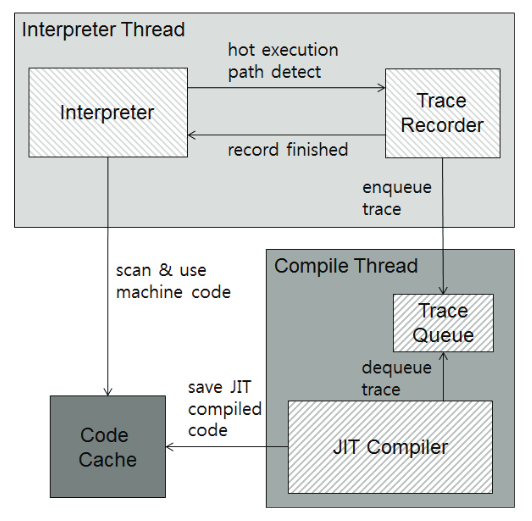
\includegraphics[scale=0.5]{images/dvm-threads.png} 
\caption{The principle of the two DVM threads. Source:\cite{oh2012evaluation}}
\label{fig:dvm-threads}
\end{center}
\end{figure}
\newpage
Depending on the different implementation of a JVM, it differs which type of JIT compiler mechanism is used.
For this thesis the Oracle JVM HotSpot is used, which has a method-based JIT compiler as default.
It is also possible to use another JIT mechanism in the HotSpot JVM triggered by parameters during the VM start.
The method-based JIT works as mentioned above, it compiles the most called methods into machine code.~\cite{kotzmann2008design}
Those methods are called hot spots, which are also responsible for the name of the virtual machine.~\cite{paleczny2001java}
\\
Both virtual machines are providing a garbage collector, which is responsible for the memory management of the byte code.
Same as the principle of own instance of the Dalvik virtual machine per process, which is being explained in Section~\ref{sec:android-internals}, every process also has its on instance of a garbage collector on Android.
It is a mark-and-sweep garbage collector that only collects the objects that are not referenced any more in the application heap.
The shared heap, which is part of the Zygote process, and which is also described in Section~\ref{sec:android-internals}, has its own garbage collector.~\cite{maia2010evaluating}
\\
Although both virtual machines are using Java as programming language, Dalvik lacks of some libraries that are available for the JVM and vice versa.
In Section~\ref{sec:migration:migration-of-basex-to-android} the used libraries of \textsc{BaseX} are analyzed and investigated which of them are supported by the DVM.\\
A general statement about both virtual machines could not be made, because they differ in a lot of aspects.
Especially that the DVM has been created for the mobile context and can only be ran on Android devices\footnote{There exist some community projects which are aiming to port the Dalvik VM to other platforms like Linux x86 for example: \url{http://www.android-x86.org/}}.



\subsection{Comparison of the two bytecode formats}
\label{sec:comparison-of-the-two-bytecode-formats}
Both virtual machines differ in their format of the executable files.
On one side there is the Java Archive File (JAR) for the JVM and the Davlik Executable (\textit{dex}) on the other side.
The \textit{dex} is being packed into an Android Application package file (\textit{apk}) which can be executed by the Android operating system.
A JAR file is an archive which includes the compressed class files, this class files are being build out of the Java source code by using the javac compiler.~\cite{pugh1999compressing} 
An \textit{apk} file is also an archive file, but it does not only include the executable program, it also includes the meta information and resource files.
Although an Android application is an \textit{apk} file only the format of the \textit{dex} file is outlined here, due to the fact that the DVM executes those files.
A \textit{dex} file is created by using a tool which compiles Java class files into \textit{dex} files.
This tool is called \textit{dx} and it is part of the Android software development kit.
Picture~\ref{fig:create-apk} illustrates the flow of an \textit{apk} creation, which differs to the creation of a JAR file by creating the \textit{dex} files out of the class files.\\
\begin{figure}[h]
\begin{center}
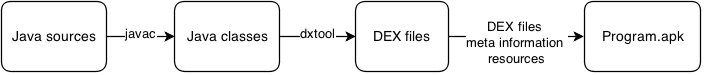
\includegraphics[scale=0.55]{images/create-apk.png} 
\caption{The creation flow of an \textit{apk} file.}
\label{fig:create-apk}
\end{center}
\end{figure}

Having a closer look at the \textit{dex} files and comparing them to the JAR files shows that they differ in various ways.
The first thing that comes in mind is that a JAR file contains a class file for every class.
And compared to this a \textit{dex} file combines all specific information into one field.
This is realized by just having one constant pool, in which all constant values of all classes are stored.
These constants are:
\begin{description}
  \item[string\_ids] Sorted list of all string identifiers
  \item[type\_ids] Sorted list of all identifiers of classes, arrays or primitive types
  \item[proto\_ids] Sorted list of all prototypes
  \item[field\_ids] Sorted list of all identifiers for the used fields
  \item[methods\_ids] Sorted list of all methods used by the \textit{dex} file
\end{description}
Thinking about an interface which is used very often in a project can display what an advantage of one shared constant pool gives.
Looking at Image~\ref{fig:jar-dex} demonstrates that every class which uses this interface has to have its own reference in its own constant pool.
\begin{figure}[h]
\begin{center}
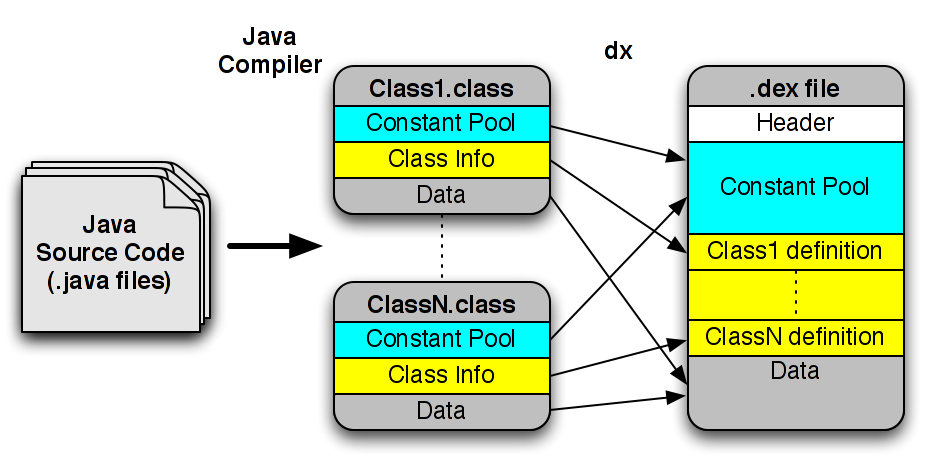
\includegraphics[scale=0.41]{images/jar-dex.png} 
\caption{The difference between a jar and a \textit{dex} file. Source:~\cite{enck2011study}}
\label{fig:jar-dex}
\end{center}
\end{figure}

In general it can be said that \textit{dex} files are smaller than their equivalent JAR files, because of the shared constant pool.~\cite{bornstein2008dalvik}
An advantage of the creation chain of a \textit{dex} file is that it is theoretically possible to create a \textit{dex} file out of every jar archive.
The problem hereby is that Android does not support all Java libraries that the JVM supports, but this can be done by using the above mentioned dx-tool. 
As mentioned before, this \textit{dex} file is executed by the Dalvik virtual machine, but it is not the Android application.
An Android application is the \textit{apk} that includes also user interface related information and other resource files, like images or sound.

\subsection{\textsc{BaseX} internals}
\label{sec:migration:basex-internals}
Although \textsc{BaseX} can be executed on every system that offers an implementation of the Java virtual machine, it has its specialties depending on the operating system that is used.
This is the case if there is something about storing files on the file system.
\textsc{BaseX} stores its databases and configuration files in a folder in the home directory of the user.
This folder is created by the database if it does not exist yet.\\
Hence, \textsc{BaseX} has to figure out on which operating system it is running.
After \textsc{BaseX} knows the operating system it stores some operating system related values in a static class, which is called \textit{Prop}. 
This class needs to be adjusted during the migration.
One value in this class is used to know if the path name is case sensitive, which is only the case for a Linux or Unix operating system and not for Windows or Mac.
To store its databases inside the folder in the directory of the home directory of the current user \textsc{BaseX} needs the absolute path to this specific folder.
Therefore the Java system method \textit{System.getProperty(``user.home'')}, which returns the absolute path to the users directory on a normal JVM, is used.\\
Another difference between Windows and other Unix based operating system is that Windows uses a backslash ``\textit{$\backslash$}'' as path separator instead of a usual slash.
This information is also stored in the above mentioned \textit{Prop} class by using the Java system method \textit{System.getProperty(``line.separator'')}.

\subsection{Android internals}
\label{sec:android-internals}
As shown in the Sections~\ref{sec:migration:comparison-of-the-two-virtual-machines} and \ref{sec:comparison-of-the-two-bytecode-formats} the two virtual machines and their corresponding bytecode formats differ.
However, Android has some other specialties about its internal processing.
The Android operating system is a Linux based operating system aimed to run on mobile devices.
Therefore it has been created as a Linux fork of the 2.6.*\footnote{Since Android version 4.* a Linux kernel 3.* is used} kernel and it is has been especially designed for the mobile context.
Which includes special focus for the resource consumption, because most mobile devices provide not the same resources as a normal desktop PC or a notebook.
As shown in Section~\ref{sec:migration:comparison-of-the-two-virtual-machines} an Android application is executed on the Dalvik virtual machine.
Here it need to be said that every application runs its own Dalvik instance, by forking the main Dalvik instance into an own Linux process.
Here sets the Android policy in, that every application is independent from every other application and is executed in its own process, which is called sandbox.
This principle is also applied for the location of all files the application needs and uses.
An application is similar in its rights and processing to a user in Linux, every application is its own user and has its own home directory.
This directory can only be accessed by the owning application and is located in the /data/data system directory.
This directory can include an own SQLite3 database, cache directory, shared preferences\footnote{Android framework that provides a mechanism to store primitive data types.} and every type of private data.
The aspect of security is the reason for this solution as well as the stability of the application, considering the own Dalvik instance.
This is called the \textit{principle of least privilege} which specifies that as less as possible privileges are given to the application.
Therefore an application developer has to specify which privileges its application needs, for example Internet access or the possibility to write on the external SD-card.
It is possible that applications can communicate with predefined Inter Process Communications (IPC) but it is not possible to manipulate other applications.
This can be omitted by granting an application root privileges, but usually this is not possible on normal devices.
Hence, confidential data should also be encrypted, because it is theoretically possible to access the data in the private directory.
It also need to be said that every operation which reads or writes to one of the above mentioned directories or files is an input output (IO) operation.
This is always expensive in time consumption and should be done as little as possible.
Image~\ref{fig:zygote-and-app} illustrates the principle that every application works in its own sandbox.\\
\begin{figure}[h]
\begin{center}
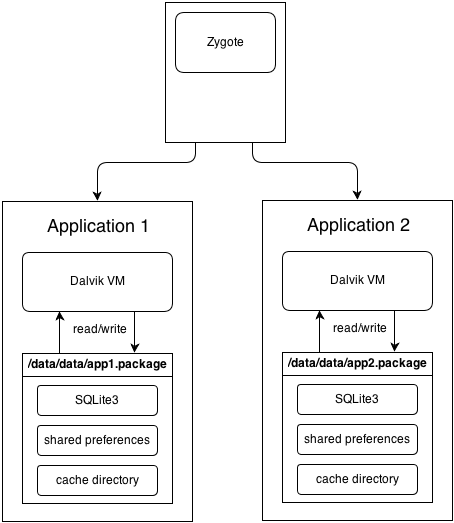
\includegraphics[scale=0.75]{images/zygote-and-app.png} 
\caption{Illustration of the Android application architecture}
\label{fig:zygote-and-app}
\end{center}
\end{figure}
\newpage
The main Dalivk instance, which is the root parent for all forked virtual machines, is called Zygote and it is started by the boot up process of Android.
Zygote is designed to load and initialize the core library classes so that every forked instance does not have to do this.
This is compared to starting a new virtual machine a speed improvement and saves memory, because not every VM instance have to has its own core libraries loaded.
This can be done because the core libraries are all read only and shared by all Dalvik instances.\cite{ehringer2010dalvik}
Another difference to the usual Linux operating system is that Android uses the Bionic libc which is a special from Google developed library for Android, which has its own pthread implementation.
This library is especially designed for the mobile context and the Android environment which improves the speed of forking the Dalvik virtual machine too.~\cite{brady2008android}

\section{Migration of \textsc{BaseX} to Android}
\label{sec:migration:migration-of-basex-to-android}
After analyzing both platforms the \textsc{BaseX} database code need to be examined too.
Like it has been mentioned in Section~\ref{sec:migration:comparison-of-the-two-virtual-machines} the Dalvik virtual machine does not support all class libraries that are supported by the JVM.
\textsc{BaseX} is written in the Java programming language and aims to be executed on virtual machines that are implemented by using the JVM specifications.
Therefore it is not possible to transform the \textsc{BaseX} jar file into a \textit{dex} file, using the dx-tool, and execute it on an Android device.
On the other side the DVM offers class libraries that the JVM does not support or knows.
These libraries do not intent to replace not supported Java class libraries, their purpose is to provide special Android related methods, for example logging or tracing of method calls as well as accessing hardware components of a mobile device, sensors or the mobile network for example. 

\subsection{Analyzing the libraries used by \textsc{BaseX}}
\label{sec:migration:analyzing-the-libraries-used-by-basex}
\textsc{BaseX} is a big project which includes up to 60 packages and more than 1300 classes, interfaces and abstract classes.
For this reason the examining of the used libraries and the dependencies a special tool was used.
It is called Class Dependency Analyzer (CDA)\footnote{http://www.dependency-analyzer.org/} and offers all needed possibilities for the mentioned task.
Parsing the whole \textsc{BaseX} project lists the used Java class libraries and external libraries.
This list gives 54 packages that are part of the Java class library or an external library used by \textsc{BaseX}.
It has to be supposed that none of them are known to the Dalvik virtual machine.\\
Most of them are subpackages of packages and it can be expected that if a main package is not supported by Android the subpackage is also not. 
This assumption reduces the external packages to a number of 16, which is compared to the before mentioned 54 packages an easier to analyze amount.
Looking at the Android documentation the main packages that are not supported are just the two graphical user interface (GUI) related packages:
\begin{itemize}
  \item java.awt\footnote{except the subpackage java.awt.font that provides two classes: NumericShaper and TextAttribute.}
  \item javax.swing
\end{itemize}
All others are full or partially supported by the Java language of the Dalvik VM.
The reason why the packages awt and swing are not supported is that Android uses its own GUI libraries and framework.
The Android provided GUI elements can either be written as Java code or can be defined in XML layout files.
The framework offers everything that is needed to build an application with a graphical user interface.\\
Supporting the main packages does not mean that all subpackages, classes or even methods that are used from other libraries are also known by the DVM.
Therefore more investigation needs to be done in order to get a better overview of the supported packages.
To get a clearer statement about the situation, the subpackages are also being checked if they are supported by the DVM or not.
The result of this investigation is that javax.xml is supported, but not the following subpackages:
\begin{itemize}
  \item javax.xml.crypto.dom
  \item javax.xml.crypto.dsig.dom
  \item javax.xml.crypto.dsig.keyinfo
  \item javax.xml.crypto.dsig.spec
\end{itemize}
Even if all packages and classes of \textit{javax.xml.crypto} are part of the Java standard edition they are not available for Android development.
All classes inside this packages were only used by one \textsc{BaseX} package which is called \textit{org.basex.query.\-util.crypto}.
This package is used to implement the XQuery cryptographic module that provides functionalities to en- decrypt, sign and validated signed XML data.
The only class that uses this package is the FNCrypto class which is used to provide the cryptographic module functionalities in XQuery.
These are XQuery functions which are:
\begin{itemize}
  \item hmac(string,string,string[,string])
  \item encrypt(string,string,string,string)
  \item decrypt(string,string,string,string)
  \item generate-signature(node,string,string,string,string,string[,item][,item])
  \item validate-signature(node)
\end{itemize}
To provide these five XQuery functions on Android, the \textit{javax.xml.crypto} package need to be migrated to Android too.
Another possibility to support these XQuery functions would be the using of other cryptographic classes which are provided by Android.\\
All other subpackages are supported by the Android platform.
For clarification not all methods that are provided by every used library are checked if they are available on Android, this would be to much effort, thinking about the amount of available classes.
Nevertheless this could be figured out in Section~\ref{sec:migration:creating-a-basex-android-library} and Section~\ref{sec:migration:problems-during-the-migration} outlines the methods which are not supported by some Android versions.

\subsection{The Android project structure}
\label{sec:migration:the-android-project-structure}
For developing Android applications an Android project need to be set up.
An Android project is a structure of special folders and predefined files, like code, resource and build files.
There are three types of Android projects, they differ in their functionalities and intentions.\\
The first is the type of project that needs to be created if an executable application is the goal of the development process.
As a result of this an installable \textit{apk} file will be created by the build process.\\
The seconds type of Android project is the so called Test project.
This type of project aims to test executable Android projects by providing an Android testing framework with unit test, using the Java unit test framework Junit.
Both projects have the same structure of folders and files.\\
The third project type is the library project which goal it is to be a library that can be used by every other Android project.
The difference to a normal Android project is that this project is not being build into an \textit{apk} file, it is being used by other Android projects which pull it in their \textit{apk} and build it with their code.
Depending on the Android API level an Android library differs from a usual Java library, by the fact that the Android library is not compressed into a jar archive.
This feature has been added in Android versions higher than API level 14, Android 4.0 codename Icecream Sandwich.
For older versions, before this API level, the library files were pulled into the project and compiled into the corresponding \textit{dex} file.\\
If a new Android application is developed it is not necessary to setup the right project structure by hand, therefore Android provides a Software Development Kit (SDK).
This SDK provides tools and utilities to create every type of Android project, it includes build, debug, trace and test tools.
With this SDK, which is also called Android Developer Tools (ADT), it is possible to create Android applications written in Java.
As it was mentioned in Section~\ref{sec:comparison-of-the-two-bytecode-formats}, the code that is translated into bytecode for the Dalvik virtual machine is written in the Java programming language.
Though, it is also possible to write code in C++ and compile it into native code, like it is done by the, in Section~\ref{sec:migration:comparison-of-the-two-virtual-machines} referred, JIT mechanism.
Therefore Google provides an Android Native Development Kit (NDK), that offers tools and a compiler to translate such native code.
If a project has been created there are seven given folders, shown in Table~\ref{tab:android-project-folders}.
\begin {table}[htpb] 
  \centering
\begin {tabular} {|l|l|}
	\hline
	src/&Contains the Java source code files\\
	\hline
	bin/&Contains the compiled output file\\
	\hline
	jni/&Contains C++ native code created by using the NDK\\
	\hline
	gen/&Contains automatic generated Java files\\
	\hline
	assets/&Is used for every kind of file, is packed into the \textit{apk} file as it is\\
	\hline
	res/&Contains all resource files\\
	\hline
	libs/&Contains private libraries\\
	\hline
\end {tabular}
\caption {Android project folders generated by the SDK.}
\label {tab:android-project-folders}
\end {table}

The files that will be appearing by creating an Android project are four build files that hold information for the build system to create the \textit{dex} files and the \textit{apk} archive.
Another file that is being created is the \textit{AndroidManifest.xml}.
This XML file is important for the application and the Android operating system.
It is used to specify the API level, the name and other specific information of the application.
In this file it is also possible to grant privileges to the application that are needed for specific functionalities.
For example accessing the Internet or writing on the external storage card.
Used libraries are also defined in this file, but if a library need some privileges and defines them into its own mainfest file, they are not granted by Android.
Therefore it is necessary to grant privileges in the Android project and not in the library project because those are being ignored.


\subsection{Creating a \textsc{BaseX} Android library}
\label{sec:migration:creating-a-basex-android-library}
For the migration of \textsc{BaseX} to the Android operating system a library project has been created.
The reason to make \textsc{BaseX} as Android library, as in Section~\ref{sec:migration:the-android-project-structure} explained, is that Android libraries can be used by many other projects.
After creating the library project all \textsc{BaseX} files have been copied to this project.
After this operation the GUI packages have been removed, those packages are \textit{basex.gui} and all subpackages.
As a result of this the depending classes of the GUI have also been removed, those are also not necessary because the \textsc{BaseX} Android library should not provide a graphical user interface.
Afterwards the not supported \textit{javax.xml.crypto} packages and the dependent class \textit{FNCrypto} have been removed.
Therefore it not possible to use the cryptological XQuery function in this \textsc{BaseX} Android version.\\
The result of removing all not supported packages, classes and libraries is that it is now possible to compile \textsc{BaseX} to an Android \textit{dex} file.
Although it is not possible at this moment to execute \textsc{BaseX}, because of some constraints mentioned in Section~\ref{sec:android-internals} and not facing the fact that an Android library is not executable.\\
In a usual Linux environment \textsc{BaseX} stores all its database files in a directory in the normal user directory.
This means executing \textsc{BaseX} on Android without adjusting the directory to store the databases, would not work.
\textsc{BaseX} receives the name and location of the home directory of the user by calling the Java function \textit{System.getProperty(``user.home'')}, which works well with the JVM.
Using this function on Android gives an empty string and results in \textsc{BaseX} trying to save the database in the root directory, what is impossible, because of the Android right system explained in Section~\ref{sec:android-internals}.
To avoid this behavior the above mentioned function need to be replaced.
The path where the data has to be stored has to be a directory that only the application can access.
Every application receives one directory with the given constraint from Android.
This is where it is installed as well as where the application stores its data.
Additionally to this it is possible for an application to read or write on external storage, but this is not protected by the operating system which means that every application can access and modify those files.\\
The problem by using the private application directory is that \textsc{BaseX} should be a library project and it should be usable by every other Android project.
So it is impossible to say how the directory is named and to locate where the database files have to be stored before even knowing how the application, which uses the \textsc{BaseX} library, is called.
The explanation for this is that an Android application receives its directory by the name of its main package and not by the name of the library main package, so that more than one application can use this library.
This is a issue that has to be dealt with, which is illustrated and discussed in Section~\ref{sec:migration:problems-during-the-migration}.
Hence, it is necessary to tell the library this location and use this instead of its own package name.
To implement this a class has been created which is an entry point for the library and is the first instance when the \textsc{BaseX} Android library is used.
This class creates an object of the library and needs the package name of the application as an argument for the method that returns an instance of its object.
To create the object the Singleton pattern has been used~\cite{gamma2010entwurfsmuster}.
The reason for this is that only one instance of the database can be created and used inside one application.\\
This class is called \textit{\textsc{BaseX}Database} and creates a \textsc{BaseX} Context object by calling a constructor that has been added to the Context class.
The newly created Context constructor checks if the given directory is available and if it is possible to read and write to this directory.
Is it the first time the constructor of the class is used, it creates a directory which is called \textit{BaseXData}.
All databases created and used by this Android application are stored inside this directory.
This directory is only accessible from this application~\footnote{Assuming the application is executed on a non rooted devices.}.
At this moment it is possible to use \textsc{BaseX} as an Android library and it would create the needed \textsc{BaseX} directory.\\
To provide the \textsc{BaseX} operations the above mentioned class has been extended by additional methods which can be used for this purpose.
All are implemented by using the above mentioned Context object, which means every operation is executed on this object.\\
After this migration it is possible to use \textsc{BaseX} as it can be done on every usual PC which provides an implementation of the JVM.
Except the cryptographic XQuery function, the \textsc{BaseX} Android library offers all functionalities like the normal \textsc{BaseX} desktop version offers.
The Android principle that every application works in its own sandbox is also being kept.
With this solution every application has its own \textsc{BaseX} database in its own directory, an advantage could be that the database does not need to consider queries that are coming from another applications and their synchronizations.\\
However, in the next section an alternative solution to this is provided by implementing the client/server mechanism of \textsc{BaseX} in Android.
The advantages and disadvantages of the library implementation are outlined and investigated in Chapter~\ref{cha:analysis}.
For the validation and performance messuarment a test application of the \textsc{BaseX} Android library has been written and its execution performance analyzed, illustrated in Section~\ref{sec:analysing-the-execution-performance}.

\subsection{Providing a \textsc{BaseX} Android server client solution}
\label{sec:migration:providing-a-server-client-solution}
At the moment every application which uses the \textsc{BaseX} Android library, has its own database that saves, provides and updates the data.
One disadvantage of this solution is that other applications can not use the data inside a database of another application.
The reason for this, as mentioned in Section~\ref{sec:android-internals}, is the sandbox principle of Android applications where applications can only access their own resources and not those from other applications.
Speaking of a disadvantage could be false, because this also prevents unauthorized applications to read or modify the data of an application.
However, Android provides a mechanism which offers the possibility to provide data from one application to another.
This technique is called content provider and is used for system wide databases like the database that contains the contacts of the owner of an Android device.
Thinking of different applications that are using the same data shows that this could lead to redundant databases, which would increase the required storage size.
In addition to this, every time the data changes on one point it has to be adjusted at every other point too.
For example, when every application has its own database storing the contacts and a new contact is added, all those databases need to updated.\\
Additionally to the stand alone version of \textsc{BaseX} it is possible to use it as a client server solution.
An instance of a \textsc{BaseX} client connects to a server and sends its requests and queries to a server, which executes them and sends them back to the client.
The advantage of this solution is that the client does not have to do the execution of the database related operations.
Also the files which are containing the data, are stored and managed on the server and not on the client.
Both shown advantages reducing resource consumptions at the client instance, it saves storage size as well as execution resources like CPU or RAM occupation.
But there is also a disadvantage, namely the client can only operate if there is a server available, and therefore it needs a connection to the server to send requests and receive responses.\\
As mentioned in Section~\ref{sec:overview:introduction-into-basex} \textsc{BaseX} also provides a client server solution, this has also been migrated to the Android platform.
Hereby the focus does not lie on the execution of the server on an external device, like a server on the Internet for example.
Although this is also possible and would bring a big saving of resources on the mobile device, but this would be similar to a web service which is not the focus of this thesis.
The server client architecture of the Android \textsc{BaseX} version is to have one central database on one place and one instance of a server that handles all database operations.
In contrast to the, in the section before created, Android library there is only one place on the device where the database files are being stored.
If an application wants to use \textsc{BaseX} as a database it uses the client and sends its operations to the server, which is executed on the same device, and then receives the results.
To achieve this Android provides Inter Process Communication (IPC) mechanisms which are offering the possibility to communicate with different applications.\\
However, the client server version of \textsc{BaseX} uses the network and the TCP protocol to do the communication between server and clients.
This technique has also been used for the Android solution of the client and server implementation.
Additionally the server has been created as an Android service.
An Android service is a process which is executed in the background and is thus the last instance which is killed by Android process management.
The reason to implement the server as an Android service is the process management of the operating system and the execution of the service in the background of the device.
The constraint of available RAM forces the Android process management to kill the not needed application and free their used spaces in the RAM.~\cite{developers2011android}
This can not be controlled, and the server has to be available all the time, so that an application can do its operation on it.
The Android operating system tries to keep the service as long as possible alive, depending on different criteria and even it is being killed, for example by the user, it tries to restart it.
A service does not provide a graphical user interface and to communicate with it also IPCs are used, therefore an application has been written, to start and stop the server service.
This application is also the sandbox where the server stores its data, the application as well as the background service are executed in this sandbox.
The data is stored in this sandbox, so no other application can access the data inside it, therefore the server is used.
To achieve this goal \textsc{BaseX} uses, as well as the desktop version, the network for the communication with the clients.
Specifically the client application does not need to implement IPCs, they send their requests via the network to the server and also receive the responses through the network.
A graphical illustration of the principle is shown in Figure~\ref{fig:server-client-android}.

\begin{figure}[h]
\begin{center}
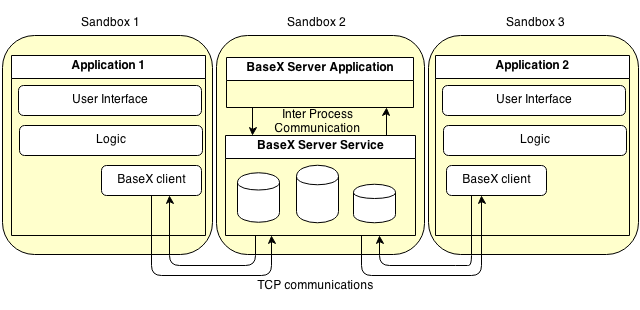
\includegraphics[scale=0.6]{images/basex-server-client.png} 
\caption{The principle of the \textsc{BaseX} server client communication in Android.}
\label{fig:server-client-android}
\end{center}
\end{figure}

Every request and operation, which uses the \textsc{BaseX} server client model, happens on the device and thus there is no saving in execution resources, only in storage capability if different applications are using the same data.
The implementation of the client server mechanism for Android has been done to illustrate that it is possible to have a server and client of \textsc{BaseX} running on one device.
The implication of this section is that it is also possible to have an external server which provides the data and the execution of the operations, which saves the above mentioned resources at the client.
The only ways to provide application data to another application are the so called content providers of Android.
The \textsc{BaseX} client/server implementation could also be seen as an alternative for the present Android content providers.\\
\\
Additionally the \textsc{BaseX} Android client as well as the library implementation are both implementing the same interface, so it is easy to replace one version with the other.
This makes it easy to replace the library with the client solution if the resources have to be stored somewhere else, for example on an external server.



\section{Problems during the migration}
\label{sec:migration:problems-during-the-migration}
There occurred several problems during the migration of \textsc{BaseX} to the Android operating system.
The first problem which was discovered, was the in Section~\ref{sec:migration:analyzing-the-libraries-used-by-basex} mentioned lack of some included libraries, that are not supported by Android.
To solve this issue they have been removed and their functionality has been deprecated.
This has been done, because those specific functionalities are not required for a first runnable \textsc{BaseX} Android version.
This also applies for all graphical user interface components, which have also been removed, because they are not necessary for an Android library.\\
Another problem was the location of the \textsc{BaseX} database directory on the Android device.
This need to be, as described in Section~\ref{sec:android-internals}, the \textit{/data/data/app\-lication-package-name} directory.
The problem hereby is that one of the goals of the migration is that the database is a library and not a standalone application.
In the Android operating system the name of the private directory of an application depends on the name of its main package.
This is only available if there is an Android application, a library does not offer this possibility, so it is not possible for a library to get the name or location of its private directory.
The only way to get the package name of the application, except for hard coding, is to get the application context and extract the name there.
This bears another problem, though only applications have a context, libraries not, which also need to be considered. 
A possible way, could be to pass the context to the library, but then the library holds the context which it does not need and it will maybe not freed from the garbage collector, due to the mark-and-sweep garbage collector mechanism, described in Section~\ref{sec:migration:comparison-of-the-two-virtual-machines}.
Also the library would only need the application context to receive the application name and by using this the name and location of the private directory.
As above mentioned, holding an Android context massively slows down an Android application, so this is not the way how it has to be solved.
The alternative is to pass a string holding the application name to the constructor of the library, because it only needs the name or the location of the data/data directory to access it.
Therefore the context has been used before creating a library instance to receive the needed directory name and this is passed to the library through the constructor.
This string is then used by the library to generate the needed directories, which can be done by the library, because it belongs to the application that uses it.
The result of this is that the library is executed in the same sandbox like the application and it has the corresponding rights.
%This is also the way how it is done in the \textsc{BaseX} library, as it was described in Section~\ref{sec:migration:creating-a-basex-android-library}.\\
An issue with this solution is that the user directory which is used in \textsc{BaseX} is a static string value initialized by the start of \textsc{BaseX}.
All static values used by \textsc{BaseX} are initialized at start-up in the static class \textit{Prop}.
And right after the start \textsc{BaseX} uses this value from this class in several places in the code.
Which means that it need to be changed before it is used anywhere in the code.
For this reason a trick has been used to initialize the value before the constructor calls another constructor.
In the \textsc{BaseX} \textit{Context}\footnote{This is the \textit{BaseX} Context class, and not the above mentioned Context class provided by Android.} class the constructor which calls the actual constructor has been changed to initialize this value as a parameter.
This results in the cycle of constructor calls, that the constructor which is called initializes the static values before calling the next constructor in the chain.
The corresponding Java code can be seen in Listing~\ref{lst:context-constructor}.
The reason that the file separator is not determined by using the available system method \textit{System.getProperty(``line.separator'')} is that the separator is the same as in Linux.
Namely it is the normal slash ``/'' and not a backslash as it is implemented in Windows operating systems.

\lstset{language=Java,
   basicstyle=\footnotesize,
   keywordstyle=\color{blue!80!black!100},
   identifierstyle=,
   commentstyle=\color{green!50!black!100},
   stringstyle=\ttfamily,
   breaklines=true,
   numbers=left,
   tabsize=2,
   numberstyle=\footnotesize,
   frame=single,
   backgroundcolor=\color{blue!3},
}
\begin{lstlisting}	[captionpos=b, captionpos=b, caption={The constructor of the BaseX context class.}, label=lst:context-constructor] 		        	   
public Context(String data_dir) {
  this(true, (Prop.HOME = data_dir + ``/''), (Prop.USERHOME = data_dir + ``/''));
        	
  File dir = new File(Prop.HOME + ``BaseXData'');
  if(!dir.exists()) {
    if(!dir.mkdir()) {
     android.util.Log.i(``BASEX'', ``CREATING BASEX DIRECTORIES'');
    }  
  }
}
\end{lstlisting} 


Another issue which occurred during the migration, was that \textsc{BaseX} uses a lot of the Java string function \textit{isEmpty()}, which is not available at an Android API-level lower than 9.
The same applies for the \textit{copyOf()} method in the \textit{java.util.Arrays} Java package.
This was solved by not supporting API-levels lower than 9 with the created \textsc{BaseX} library.
According to the official Android homepage only 1.7\% of the devices that are currently in circulation have an API-level lower than 9.\footnote{\url{http://developer.android.com/about/dashboards/index.html}}
The consequence of this would be that developers can only create applications that are executable on Android devices using an API-level higher than 9, when using the \textsc{BaseX} library.
To assure that no application, that is build on Android version lower than 9, uses the \textsc{BaseX} library the Manifest file of the library has been adjusted.
This is one of the cases where the Manifest file of a library is used to determine the minimum Android version.
Other constraints specified inside this Manifest file, like write permissions for example, are being ignored, as it was mentioned in Section~\ref{sec:migration:the-android-project-structure}.


\chapter{Analysis of the ported \textsc{BaseX} Android version}
\label{cha:analysis}
The following chapter outlines how the migrated \textsc{BaseX} Android database is analyzed.
The focus at this part lies on the evaluation and the performance of the library.
First the specification of the test devices is outlined and an estimation is made to show how the performance of the various devices differ.
Therefore different benchmarks has been executed to approximate the distinctive hardware properties and their execution times.
In the next chapter is shown that the migrated database works without errors and failures on the Android mobile platform using a real devices.
For this purpose different unit test has been also migrated to test the functionality.
After evaluation the functionality the performance has been investigated.
An overview of the performance an XML benchmark set, which is especially designed to test the performance of XQuery executions, has been used.
\section{Evaluation of the test devices}
\label{sec:evaluation-of-the-test-devices}
For the measurement of the performance two devices are being used.
First, for testing the \textsc{BaseX} mobile version an Android Tablet PC Samsung Galaxy Tab 2 10.1 and for the normal \textsc{BaseX} version a Lenovo Thinkpad laptop have been used.
Their technical specifications can be seen in Table\ref{tab:test-dev-specs}.
\begin {table}[htpb] 
  \centering
\begin {tabular} {|r|r|r|r|r|r|}
  	\hline
	&CPU&RAM&filesystem&operating system\\
	\hline
	Laptop&Intel Core2 Duo CPU L7100&2 Gb&ext4&Arch Linux\\
	&1.2 GHz&&&(3.12.0)\\
	\hline
	Tablet&Dual-core Cortex-A9&1 Gb&ext4&Android\\
	&1 GHz&&&(4.0.3)\\
	\hline
\end {tabular}
\caption {The technical specifications of the two devices, used for benchmark testing.}
\label {tab:test-dev-specs}
\end {table}

Looking at this table it can be seen that the only similarity of both systems is that they are using the same filesystem, which is ext4, which is short for fourth extended filesystem.
The RAM of the laptop is the double amount of the tablet available RAM and both devices have a dual core CPU with around 1 GHz.
Even if the specifications are not so much differ on the first look, their performance varies in some factors.
Therefore a measurement of the input/output (IO) and CPU speed of booth devices has been made in Section~\ref{sec:evaluation-of-the-test-devices} to get a clearer look how the devices differ.


%\section{Evaluating the working \textsc{BaseX} Android port}
%\label{sec:evaluating-the-working-basex-android-port}
%\textbf{TODO}\\
%In this section will be shown that the created \textsc{BaseX} Android port works and fit all requirements.
%For this purpose the given JUnit tests were been migrated to Android too.
%This shows that all functions work like they work on the standard Java version.
The two devices which have been used to benchmark \textsc{BaseX} are totally different and not just in the fact that one is laptop and the other a tablet PC.
They differ in many hardware aspects, but there are two different factors, that are interesting to identify a systems speed and are used for the given purpose.
These are the CPU speed and the input/output (IO) speed, where IO speed is a headline for different operations.
Broadly speaking it can be said that the IO speed can be divided into read and write operations.\\
To measure this values the benchmark tool Bonnie++\footnote{\url{http://www.coker.com.au/Bonnie++/}} is used.
This tool executes different operations and measures how many of these operations can be executed in one second.
It tests sequential output, sequential input, random seeks, sequential create and random create.\\
The sequential output represents the write speed of the system, Bonnie++ uses three different methods to measure this value.
First it writes one character after another by using the \textit{putc()} systemcall. 
After this operation it writes whole blocks with the size of 8192 bytes by using the write() systemcall and than calling the close() systemcall.
The last test in this category is the rewrite test and differs from the write test, that the file is not closed after writing.
Therefore one block write comply with 8192 \textit{putc} calls and is way more effective and faster than writing single characters.
The next test is to measure the random seek operations per seconds, which means how often the read/write position can be changed.
It also measures the latency which represents the rotation speed of the disk, but this is obsolete because both systems have flash storage and so there is no revolution per minute to measure.
Bonny is written in C++ and is available on most Linux distributions, but to use it on Android it is necessary to build it from its sources by using the, in Chapter~\ref{sec:migration:the-android-project-structure} mentioned, Android Native Development Kit (NDK).
This provides a cross compiler which makes it possible to build C++ code for Android.
For the execution of the benchmarks the version 1.96 from Bonnie++ has been used.
The results of these test executions can be seen in table~\ref{tab:bonnie-results-out}.
%\begin {table}
%\begin {tabular} {|r|r|r|r|r|r|r|r|r|r|r|r|r|}
%	\hline
%		&\multicolumn {3} {|c|} {Sequential}&\multicolumn {2} {|c|} {Sequential}&Random&\multicolumn {3} {|c|} {Sequential}&\multicolumn {3} {|c|} {Random}\\
%		&\multicolumn {3} {|c|} {Output}&\multicolumn {2} {|c|} {Input}&Seeks&\multicolumn {3} {|c|} {Create}&\multicolumn {3} {|c|} {Create}\\
%	\hline
%		&K/sec&K/sec&K/sec&K/sec&/sec&/sec&/sec&/sec&/sec&/sec&/sec&/sec\\
%	\hline
%	Laptop&201&62180&23850&907&98239&1161&17134&137752&13032&19442&170028&11774\\
%	\hline
%	Tablet&5&20828&8756&596&23768&475.6&39&361&167&42&391&238\\
%	\hline
%	\hline
%	Factors&40.20&2.99&2.72&1.52&4.13&2.44&439.33&381.58&78.04&462.90&434.85&49.47\\
%	\hline
%\end {tabular}
%\caption {Results of the Bonnie++ benchmarks.}
%\label {tab:bonnie-results}
%\end {table}


\begin {table}[htpb] 
  \centering
\begin {tabular} {|r|r|r|r|r|r|r|}
	\hline
		&\multicolumn {3} {|c|} {Sequential}&\multicolumn {2} {|c|} {Sequential}&\multicolumn {1} {|c|}{Random}\\
		&\multicolumn {3} {|c|} {Output}&\multicolumn {2} {|c|} {Input}&\multicolumn {1} {|c|}{Seeks}\\
	\hline
		&Char&Block&Rewrite&Char&Block&\\
	\hline
	Laptop&201K&62180K&23850K&907K&98239K&1161\\
	\hline
	Tablet&5K&20828K&8756K&596K&23768K&475.6\\
	\hline
	\hline
	Factors&40.20&2.99&2.72&1.52&4.13&2.44\\
	\hline
\end {tabular}
\caption {Results of the Bonnie++ in- and output benchmarks.}
\label {tab:bonnie-results-out}
\end {table}


Bonnie++ also measures the sequential and random create of a file.
Therefore it creates, queries its status and deletes a file by using the Posix systemcalls \textit{creat()}, \textit{stat()} and \textit{unlink()}.
The results of this test can be seen in Table~\ref{tab:bonnie-results-create}
\begin {table}[htpb] 
  \centering
\begin {tabular} {|r|r|r|r|r|r|r|}
	\hline
		&\multicolumn {3} {|c|} {Sequential}&\multicolumn {3} {|c|} {Random}\\
		&\multicolumn {3} {|c|} {Create}&\multicolumn {3} {|c|} {Create}\\
	\hline
		&creat()&stat()&unlink()&creat()&stat()&unlink()\\
	\hline
	Laptop&17134&137752&13032&19442&170028&11774\\
	\hline
	Tablet&39&361&167&42&391&238\\
	\hline
	\hline
	Factors&439.33&381.58&78.04&462.90&434.85&49.47\\
	\hline
\end {tabular}
\caption {Results of the Bonnie++ sequential/random create benchmarks.}
\label {tab:bonnie-results-create}
\end {table}


%\begin {table}
%\begin {tabular} {|r|r|r|r|r|r|r|}
%	\hline
%		&\multicolumn {3} {|c|} {Sequential}&\multicolumn {2} {|c|} {Sequential}&\multicolumn {1} {|c|}{Random}\\
%		&\multicolumn {3} {|c|} {Output}&\multicolumn {2} {|c|} {Input}&\multicolumn {1} {|c|}{Seeks}\\
%	\hline
%		&Char&Block&Rewrite&Char&Block&\\
%	\hline
%	Laptop (per seconds)&201K&62180K&23850K&907K&98239&1161\\
%	\hline
%	Tablet (per seconds)&5K&20828K&8756K&596&23768K&475.6\\
%	\hline
%	\hline
%	Factors&40.20&2.99&2.72&1.52&4.13&2.44\\
%	\hline
%\end {tabular}
%\caption {Results of the Bonnie++ benchmarks.}
%\label {tab:bonnie-results}
%\end {table}


By analyzing these values it can be said that the laptop is overall faster than the tablet PC.
It is well known that IO operations are the most expensive one on Android, so the achieved result is no surprise. 
But with these values it can be said that there are factors which can tell how much faster it is in specific operations.
This factors are impossible to optimize, because they are a hardware constraint and only changing the hardware can improve them, but they are still important to identify the bottlenecks of the mobile \textsc{BaseX} version.\\
Analyzing Table~\ref{tab:bonnie-results-create} and having a look at the factors shows one value which is, compared to the other factors, extremely high.
The sequential write per character is 40 times faster on the laptop than on the tablet, considering this, it is clear to avoid writing by character instead by block.
Writing by using the block mechanism is just three times slower on the tablet.
The sequential reading of a single character is at the tablet just 1.52 times slower than the at the notebook.
Though the factor of the block reading is quite higher than the character reading factor it is sure to use the block reading because it is much faster than character reading.
But by using block reading the factor need also be considered in the \textsc{BaseX} benchmarks later in chapter~\ref{sec:analysing-the-execution-performance}.
\\
Looking at Table~\ref{tab:bonnie-results-create} it can be seen that the sequential/random creation, reading and deleting is very slow on the Android devices compared to the laptop.
Considering this it should be avoided to often create files, because this is very slow.\\
Bonnie++ gives a good overview about how fast the two system handle their IO operations and how they differ in this aspect.
But there is also another factor which affects the speed of the execution of a program.
This is the CPU speed, it is obvious that this also differs on both test devices.
To evaluate the CPU times a Java program has been written which executes four different CPU intensive operations.
First it does the naive factorial of 5000, where naive means that it just iterates till 5000 and multiplies every step to the result.
The second test is a recursive calculation of the 100th Fibonacci number.
The third sorts an ascending ordered array of 10000 items using the bubble-sort algorithm.
This is done because this is the worst case for the bubble-sort algorithm and has a complexity of $\mathcal O(n^2)$.
The last test makes a naive test if the number 666667 is prime or not, by testing to divide the number by every candidate step by step till the candidate is the square root of the number.
All these test are very CPU intensive, because they use only arithmetic operations.
The results of these test can be seen in Table~\ref{tab:cpu-results}.
\begin {table}[htpb] 
  \centering
\begin {tabular} {|l|r|r|r|r|}
	\hline
		&Factorial&Fibonacci&Bubble Sort&Prime Number\\
	\hline
	Laptop&&&&\\
	(avg. on 1000 runs)&98.19 ms&248.63 ms&180.53 ms&15.85 ms\\
	\hline
	Tablet&&&&\\
	(avg. on 1000 runs)&491.15 ms&2336.35 ms&1045.52 ms&76.41 ms\\
	\hline
	\hline
	Factors&5&9.4&5.8&4.8\\
	\hline
\end {tabular}
\caption {Results of the CPU benchmarks.}
\label {tab:cpu-results}
\end {table}


Except the Fibonacci test it can be said that the CPU of the laptop is about five times faster than the one of the laptop.
This is like the different IO parameters a factor which could not be improved and has to be considered in the \textsc{BaseX} benchmarks as well.
These evaluation is for measuring the performance of the two \textsc{BaseX} versions and how to cope with the results achieved by two different platforms on two different devices.


\section{Analyzing the execution performance}
\label{sec:analysing-the-execution-performance}
To investigate the performance of the Android version of \textsc{BaseX} the benchmark suite \textit{XMark} has been used.
\textit{XMark} creates random XML files and has a set of twenty predefined queries that can be used to measure the execution performance of an \textit{XQuery} implementation.
It offers the possibility to choose the size of the random XML files, so that the test queries can be executed on different file sizes.
Therefore it is also being used to find the maximum supported size of a \textsc{BaseX} database on Android.


\subsection{The XMark benchmark suite}
\label{subsec:the-xmark-benchmark-suite}
The XMark benchmark suite is used to identify the speed of the \textsc{BaseX} Android version.
Therefore it offers 20 different XQueries which are designed to benchmark a XQuery implementation.
The queries are separated into different categories, where every category targets a specific aspect of query execution.
The XML files that can be generated by using XMark are all containing the same elements and every file is well-formed.
The content of the generated XML files is randomly generated by using the 17000 most frequently used words~\footnote{ignoring stop words} in the plays of Shakespeare~\cite{schmidtxmark}.
The structure of the randomly generated XML files can be seen in Figure~\ref{fig:xmark-file-structure}.
\begin{figure}[h]
\begin{center}
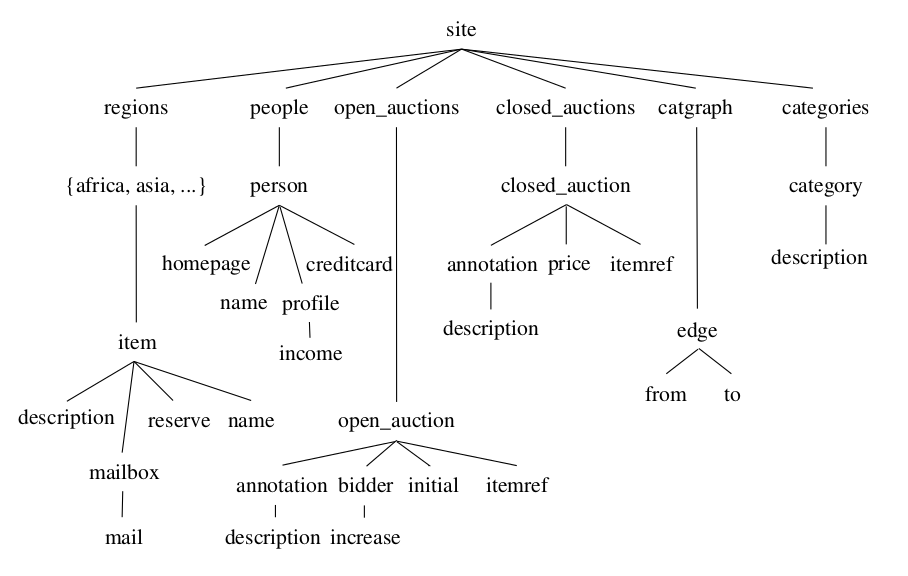
\includegraphics[scale=0.42]{images/xmark-file-elements.png} 
\caption{The structure of a generated XMark XML file. Source:\cite{schmidtxmark}}
\label{fig:xmark-file-structure}
\end{center}
\end{figure}

The size of the XML files can be chosen during the generation process of XMark.
For testing \textsc{BaseX} 15 different files were been generated.
The smallest with the size of 100 Kb followed by files with a size increasing by 100 Kb steps.
Hence, the biggest generated file has a size of 1.4 Mb.\\
The different queries can be seen in Table~\ref{tab:xmark-queries}.
\begin {table}[htpb] 
  \centering
	\begin{tabular}{r|l}
	  \hline
	  1&Return the name of the person with ID 'person0'.\\
	  \hline
	  2&Return the initial increase of all open auctions.\\
	  \hline
	  3&Return the first and current increase of all open auctions whose current\\
	  &increase is at least twice as high as the initial increase.\\
	  \hline
	  4&List the reserves of those open auctions where a certain person issued\\
	  &a bid before another person.\\
	  \hline
	  5&How many sold items cost more than 40.\\
	  \hline
	  6&How many items are listed on all continents?\\
	  \hline
	  7&How many pieces of prose are in our database?\\
	  \hline
	  8&List the names of persons and the number of items they bought.\\
	  &(Joins person, closed\_auction)\\
	  \hline
	  9&List the names of persons and the names of items they bought in Europe.\\
	  &(Joins person\_auction, item)\\
	  \hline
	  10&List all persons according to their interest; use French markup\\
	  &in the result.\\
	  \hline
	  11&For each person, list the number of items currently on sale whose\\
	  &price does not exceed 0.02\% of the person's income.\\
	  \hline
	  12&For each richer-than-average person, list the number of items currently\\
	  &on sale whose price does not exceed 0.02\% of the person's income.\\
	  \hline
	  13&List the names of items registered in Australia along with\\
	  &their description.\\
	  \hline
	  14&Return the names of all items whose description contains the word 'gold'.\\
	  \hline
	  15&Print the keywords in emphasis in annotations of closed auctions.\\
	  \hline
	  16&Return the IDs of those auctions that have one or more keywords\\
	  &in emphasis.\\
	  \hline
	  17&Which persons don't have a homepage?\\
	  \hline
	  18&Convert the currency of the reserve of all open auctions to\\
	  &another currency.\\
	  \hline
	  19&Give an alphabetically ordered list of all items along with their location.\\
	  \hline
	  20&Group customers by their income and output the cardinality of each\\
	  &group.\\
	  \hline
	\end{tabular}
	\caption {The XMark queries. Source:\cite{schmidtxmark}}
\label {tab:xmark-queries}
\end {table}


The queries are divided into various categories, which are aiming to benchmark several functionalities and concepts of XML.
Category one includes just Query 1 and tests the performance of an exact match.
The second category analyzes the behavior of the database by querying it with order constraints.
This category contains the queries 2, 3 and 4.
Casting is the purpose of the third category, which only includes Query 5.
The next category contains the queries 6 and 7, and tests the regular path expressions.
Chasing references is the topic of Category 5 that holds Query 8 and 9.
Constructing new elements and querying them is the purpose of the next category that includes only Query 10.
Benchmarking the execution of queries with a large result set by using joins is the goal of Category 7, which involves Query 11 and 12.
Query 13 is the only query in the next category, which aims to test the performance of reconstruction of a document.
Search a full text by using a key word is the purpose of Category 9 that just includes Query 14.
The next category tests the performance of deep path traversals without wildcards, this includes the Queries 15 and 16.
Category 11 includes Query 17 and investigates the performance of the database by querying missing elements.
User defined functions are the content of the next category which contains Query 18.
To investigate the performance of the database executing a query that sorts the result is the purpose of Category 13 which is achieved by Query 19.
The last category is used to test the speed of an execution of a simple aggregation by using the last query.~\cite{schmidtxmark}.

\subsection{The Results of the Benchmark Execution}
\label{sec:the-results-of-the-benchmark-execution}
To execute the XMark queries two applications have been developed, one for testing the \textsc{BaseX} desktop version and one for the Android version.
These two programs are the same except the target platform and the used \textsc{BaseX} version.
They have the same functionalities and they operate equal.
First the programs create 15 databases and add the, in the section before mentioned 15 XML files, to these databases.
After this operations the application opens one database after another and executes every XMark query on it.
Every query is executed a hundred times and the average time consumption is being calculated and stored into a file.
The result of the execution of the application using the Laptop can be seen in Figure~\ref{fig:xmark-laptop} and the result of the execution using the Tablet is shown in Figure~\ref{fig:xmark-tablet}.

\begin{figure}[!ht]
  \begin{center}
  \begin{gnuplot}[terminal=pdf, terminaloptions=color, scale=1.1]
          set title 'Laptop Steps'
	  set datafile separator ','
	  set xlabel 'Query'
	  set ylabel 'Average time in ms(100 executions)'
	  set xrange [0:21]
	  set xtics 1,1,20
	  set logscale y
	  set grid ytics lt 0 lw 1 lc rgb '#bbbbbb'
	  set grid xtics lt 0 lw 1 lc rgb '#bbbbbb'
	  set key samplen 2 spacing .5 font ',8'
	  show grid
	  set style fill solid 0.8 border -1
	  set boxwidth 0.5 relative
	  plot for [i=1:14] 'benchmarks/basex-steps-laptop-transposed.csv' u ($0+1):i title ''.i.'00kb' with linespoints
	\end{gnuplot}              
	\caption{The results of the XMark benchmark queries executed on the Laptop.}
	\label{fig:xmark-laptop}
	\end{center}
\end{figure}
\begin{figure}[!ht]
  \begin{center}
  \begin{gnuplot}[terminal=pdf, terminaloptions=color, scale=1.1]
          set title 'Tablet Steps'
	  set datafile separator ','
	  set xlabel 'Query'
	  set ylabel 'Average time in ms(100 executions)'
	  set xrange [0:21]
	  set xtics 1,1,20
	  set logscale y
	  set grid ytics lt 0 lw 1 lc rgb '#bbbbbb'
	  set grid xtics lt 0 lw 1 lc rgb '#bbbbbb'
	  set key samplen 2 spacing .5 font ',8'
	  show grid
	  set style fill solid 0.8 border -1
	  set boxwidth 0.5 relative
	  plot for [i=1:14] 'benchmarks/xmark-tablet-steps-transposed.csv' u ($0+1):i title ''.i.'00kb' with linespoints
	\end{gnuplot}              
	\caption{The results of the XMark benchmark queries executed on the Tablet.}
	\label{fig:xmark-tablet}
	\end{center}
\end{figure}

Looking at both images it can be seen that with increasing size of the database also the execution time of the test queries rises.
This was expected, because all queries have a complexity of at least $\mathcal O(n)$ and with increasing file size the amount of elements also increase.
It is also shown that the curves of both images are similar to each other, which is a sign that no unpredictable circumstances set in.
A query which is very fast on one devices and the slowest on the other or vice versa would be an example for this.
Although the graphics look very much alike they differ in one important aspect, the fact that the execution time is up to seventy times higher using the Tablet instead of the Laptop.
Even if this factor is just the highest one, the queries which are executed using the Tablet are around thirty times slower, on average, than the one executed on the Laptop.
\footnote{The complete results of all executed XMark benchmark tests of the Laptop and the Tablet are shown in Appendix~\ref{app:the-xmark-results}. There is also a table given with the factors which are showing how the execution times differing.}
This results are giving a first overview of the performance of \textsc{Basex} running on Android.
The perception that \textsc{BaseX} is faster executed on the Laptop was anticipated, by just considering the lack of hardware resources at the Tablet shown in Section~\ref{sec:evaluation-of-the-test-devices}.
Remembering the fact that, for example, the CPU speed is circa five times higher on the Laptop than on the Tablet it need some investigation how such factors like the seventy times higher execution time are being achieved.
Another interesting insight is the fact that the execution time is sometimes faster with a bigger database than a small one.
This only affects the benchmarks made using the Tablet device.
In general it can not be said how the above mentioned circumstances occur.
Hence, more research needs to be done with the \textsc{BaseX} Android version, which is shown in the next section.

\subsection{Identifying the Bottlenecks}
\label{sec:identifying-the-bottlenecks}
With the Android SDK various development tools are provided.
On of them is Traceview, which offers the possibility to record a specific part as source code of an execution of an application.
Traceview provides a graphical view to analyze this records or the possibility to transform them into HTML code.
The content of such record implies every method call and its execution time, as well as the occupation of the CPU in percent and the amount of calls.
The execution times are given in microseconds which are not representing the real world time, the value represents absolute CPU occupation time.
This fact makes the recorded trace-views very valuable, because no interrupts are tampering the results.\\
All twenty XMark queries have been recorded with Traceview by executed on a database of the size of one mega byte.
Most records contain a very long list of method calls, even if they only record a small part of the code.
Therefore only the top five time consuming methods of every query have been investigated.
Summing those methods up it can be said that there is an amount of twenty methods which are the top five time consuming methods that have been recorded using Traceview.
%The five most frequent of those can be seen in Table~\ref{tab:tob-five-time-methods}.
%\begin{table}[htpb]
%	\centering
%	\begin{tabular}{|c|c|}
%		\hline
%		Occurrence&Name\\
%		\hline
%		14&query/value/node/DBNode\$4.next\\
%		\hline
%		11&io/random/TableDiskAccess.read1\\
%		\hline
%		10&query/value/item/QNm.eq\\
%		\hline
%		8&query/path/NameTest.eq\\
%		\hline
%		8&util/Compress.pull\\
%		\hline
%	\end{tabular}
%	\caption{The most time consuming methods recorded by using Traceview.}
%	\label{tab:tob-five-time-methods}
%\end{table}
%
%The leading method of Table~\ref{tab:tob-five-time-methods} is the \textsf{DBNode\$4.next} method, which is 14 times in the top five most time consuming methods of the twenty XMark queries.
%Looking at the source code of this method and the fact, that the average cycles per method call are 18 shows that there is no opportunity to optimize the \textsf{next} method.\\
%The next method is \textsf{TableDiskAccess.read1} which is eleven times in the most time consuming methods of the XMark queries.
%It is faster than the, before mentioned, \textsf{next} method, because its average$cycle \over calls$ relation is 8, which indicates that a default call lasts 8 cycles in this method.\\
%The next one in the list is the \textsf{QNm.eq} method with an occurrence of ten times and an average execution time of twenty cycles.
Traceview also records the amount of calls that every method experienced.
With this information it is possible to calculate the average time spend in one method, Table~\ref{tab:tob-five-cycle-call} shows the methods which having the highest values as a result of this calculation.
\begin{table}[htpb]
	\centering
	\begin{tabular}{|c|c|}
		\hline
		${cycle \over calls}$&Name\\
		\hline
		32592&dalvik/system/VMDebug.startGC\\
		\hline
		1121&util/Compress.unpack\\
		\hline
		277&value/node/DBNode.uri\\
		\hline
		175&query/path/IterStep\$1.next\\
		\hline
		105&util/Token.norm\\
		\hline
	\end{tabular}
	\caption{The five methods with the highest${cycle \over calls}$ value.}
	\label{tab:tob-five-cycle-call}
\end{table}

The most time consuming method is, shown in Table~\ref{tab:tob-five-cycle-call}, \textsf{VMDebug.startGC}.
This function is called only one time and executes a long time in average.
According to~\cite{vmdebug-startgc} this method is a fake method, it is implemented to display the execution of the garbage collector of the Dalvik virtual machine on the Traceview records.
Unlike most implementations of the Java virtual machine, it is not possible for the Dalvik VM to change the garbage collector mechanism.
It is possible to increase the size of the process own heap, which indirectly affects the garbage collection, by slowing it down with bigger heap size.
The available heap is hereby device dependent and increasing the size can cause crashes of the application, with out of memory exceptions.
Since the Android version 2.3, which is the minimum version for the \textsc{BaseX} Android library, the garbage collector is concurrent and does not influence the executing thread.~\cite{dubroy2011memory}
This is also the reason why it is executed only once and takes so long, it is started for one time and collects the unreferenced objects till the process is finished.
Therefore this method is being ignored, because increasing the heap size is not an option and the garbage collector is not executed on the thread which benchmarks the \textsc{BaseX} code.

%\subsection*{Analyzing the \textsf{Compress.unpack} method}
%\label{sec:analyzing-the-compress.unpack-method}
Looking at those methods, the \textsf{DBNode.uri} method is the only one of those, which provides a possibility to be optimized, by modifying the Java source code.
Unfortunately, this method is not the top time consuming method, \textsf{Compress.unpack} is the slowest executed method, recorded by traceview.
It consumes an average of 1121 cycles per call, which is compared to the other methods very slow.
The purpose of this method, inside \textsc{BaseX}, is to decompress the given byte array.
Therefore it iterates over the given byte array and decompresses all characters.
\\
The \textsf{IterStep\$1.next} method is part of an iterator and iterates to the next node.
Depending on the amount of nodes, the time spend in this method and the corresponding calls to it can in- or decrease.
\\
\textsf{Token.norm} is used to normalize all whitespaces in the byte array given in the parameter of the method.
By normalizing it is meant to search for horizontal tabs, line feeds, carriage returns and spaces inside the byte array and then replaces them by an empty character.
This is done in a normal for-loop and could not be improved by changing it.
The only method, that has the potential to be optimized by modifying the Java source code is the \textsf{DBnode.uri} method, which is shown in the next section.


\subsection*{Analyzing the \textsf{DBNode.uri} method}
\label{sec:analyzing-the-dbnode.uri-method}
The third most time consuming method is the \textsf{DBNode.uri} method with an average of 277 cycles per call.
Listing~\ref{lis:uri-code} shows the corresponding source code to the \textit{NSGlobal.uri} method.
\lstset{language=Java,
   basicstyle=\footnotesize,
   keywordstyle=\color{blue!80!black!100},
   identifierstyle=,
   commentstyle=\color{green!50!black!100},
   stringstyle=\ttfamily,
   breaklines=true,
   numbers=left,
   tabsize=2,
   numberstyle=\footnotesize,
   frame=single,
   backgroundcolor=\color{blue!3},
}
\begin{lstlisting} [captionpos=b, caption={The code for the uri method in the NSGlobal class.}, label=lis:uri-code] 
public byte[] uri(final byte[] pref) {
    if(stack != null) {
      for(int s = stack.size() - 1; s >= 0; s--) {
        if(eq(stack.name(s), pref)) return stack.value(s);
      }
    }
    final byte[] uri = staticURI(pref);
    return uri == null ? NSGlobal.uri(pref) : uri.length == 0 ? null : uri;
}
\end{lstlisting}
		
%An answer to this question could be that the amount of the iterations of the for loop is the highest value it can be, because nothing more happens in the loop and its complexity is $\mathcal O(n)$.
Looking at the source code of the \textit{uri} method shows that it only executes a for-loop and checks if the parameter \textsf{pref} is equal to the \textsf{NS.name} byte and if this the case the value is returned.
The method has a complexity of $\mathcal O(n)$ which results in the assumption that the for-loop is always executed in the worst case.
This would mean that every time the method is called the loop is fully iterate from the maximum size of the \textsf{NS} object till zero.
Considering the, in Section~\ref{sec:migration:comparison-of-the-two-virtual-machines} mentioned, Just In Time compiler from the Dalvik VM this part of code should be optimized by it.
Even if this part of the \textsc{BaseX} Android source code is compiled into native machine code it is still very slow, compared to the other expensive methods.
Besides the for-loop there are the \textsf{eq} and \textsf{NS.name} methods, which could produce the long execution time of this function.
The \textsf{eq} method compares the two commited byte arrays for equality, implemented by using a for-loop which iterates over the arrays and compares their bytes.
This for-loop is executed very often and there are no other method calls inside of it, so it is very obvious that this loop is compiled into machine code by the JIT optimization routine.\\
Investigating the \textsf{NS.name} method shows that this function is a simple getter method which returns the name from the index of the parameter.\\
At this place the differences between the two platforms are playing an important part, because it is best practices to use getter and setter for the normal Java environment, but it is expensive for the Android platform.~\cite{toninievlautatingandroid}
Even if the JIT compiler inlines the getter/setter calls it can be up to 30\% faster if a direct field access is used instead of the getter/setter methods.~\cite{toninianalysis}\\
In Section~\ref{sec:improving} the getter of the \textit{NSGlobal.uri} method has been replaced by direct field accesses and it is shown if it improves the execution time of Query 2 for the \textsc{BaseX} Android library.

\subsection*{Analyzing the hardware usage}
\label{sec:analyzing-the-hardware-usage}
In Section~\ref{sec:evaluation-of-the-test-devices} it has been shown, that the Laptop computes five times faster, in average, as the Tablet.
Additionally to this the write operation on the file system is up to 3 times slower on the Tablet compared to the Laptop and the read operation is around four times faster on the Laptop.
Thinking about those factors could lead to the solution that most of the bigger execution time on the Tablet is achieved by the given hardware constraints.
The created traceviews show also a often use of the \textsf{TableDiskAccess} class.
This class offers methods to store the data on the disk or to read it, therefore it uses block-wise operations.
The measured values of Section~\ref{sec:analyzing-the-hardware-usage} for the I/O operations on the test devices, illustrates that writing is three times faster on the Laptop than on the Tablet.
And reading is even more than 4 times faster compared to the Tablet device, by using block wise operations.
For the XMark benchmark test a write operation has not been executed, because the benchmarks only query the data and does not create new one which is stored permanently in the database.
Therefore no traceview shows the usage of the \textsf{writeBlock} method for example, the analyzing of the write performance of the \textsc{BaseX} Android library is shown later in this section.\\
In contrast to the write operation, the read operation is used very often.
Even it is not part of the most time consuming methods in the traceviews it is still the factor of 4 which need to be considered, always when it is being executed.\\
To measure the performance of the write operation an Android application has been created which creates databases and fills them with different data.
The provided data has been created using the provided XMark tool to create random XML files, therefore files with the size of 1, 5 and 10MB have been generated.
As well as testing the Android version of \textsc{BaseX} in its write ability the desktop version has also been tested with the same data.
The results can be seen in Table BLABLUB.

The results of the measured write operations illustrates that the Laptop is in average three times faster in writing operations than the Tablet device.
This is the same factor achieved by the evaluation of the test devices in Section~\ref{sec:evaluation-of-the-test-devices} by using block writing operations.
This realization leads to the consumption that this value is a hardware constraint and can not be optimized by changing the source code or any other software aspect.

\section{Results of the improvement}
\label{sec:improving}
%In this section is shown how the found bottlenecks can be improved and the time consumption of some functionalities are made better.
One aspect which was found as a possible improvement, by analyzing the execution times and the corresponding traceviews from Section~\ref{sec:identifying-the-bottlenecks}, is the getter and setter part.
As mentioned in Section~\ref{sec:analyzing-the-dbnode.uri-method} the use of direct field access instead of getter/setter methods improves the execution time by 30\%.
This value is shown by~\cite{toninievlautatingandroid} and is the change which has been done for the \textsc{BaseX} Android library.
The recorded traceviews have shown that especially the \textsf{DBNode.uri} has a high execution time caused by the getter calls in the for-loop.
This call accesses the \textsf{nm} byte array which is one part of tuples of name and value pairs in the container class \textsf{Atts}.
All calls to the getter and setter to these tuples have been replaced by direct field accesses in the whole \textsc{BaseX} Android library.\\
Execution of the XMark benchmark tests with this optimized version of \textsc{BaseX} on the tablet showed an improvement of up to 180\%, which is nearly three times faster as the normal version.
Especially the time consumption for the execution of queries 2, 10 and 17 have been improved.
An extensive use of the \textsf{DBNode.uri} method at those queries is responsible for this behavior.
The average improvement of this change is about 58.6\%.
Analyzing the traceviews of the improved version shows, that the average execution time of the \textsf{DBNode.uri} method has been nearly cut into half and it is not even close to the list of the top time consuming methods.
The results of the whole execution can be seen in Appendix TODO.
The replacement of the getter and setter calls at the desktop version of \textsc{BaseX} have no significant changes in the time consumption of the execution time.
The average improvement of 58.6\% is even higher than the 30\% mentioned before and achieved by~\cite{toninievlautatingandroid}.
This shows, that the replacement of the getter/setters is a technique which need to be continued in the \textsc{BaseX} library project, as well in every other time consuming Android application.
Responsible for the improvement on the Android platform is the, in Section~\ref{sec:migration:comparison-of-the-two-virtual-machines} mentioned, Just In Time compiler of the Dalvik virtual machine. 
Even if the compiler copies the getter and setter methods to the corresponding place in the code, the JIT is not able to transform them into native code, therefore they have to be replaced by direct field accesses.
Translating those accesses into native machine code is responsible for the boost of time improvement.
Looking at Figure~\ref{fig:xmark-tablet-optimized} shows that there are no significant changes in the execution time of the queries.
The Queries 8, 9 and 11 are still the slowest ones, but the overall time consumption could has been lowered.


\begin{figure}[!ht]
  \begin{center}
	\begin{gnuplot}[terminal=pdf, terminaloptions=color, scale=1.1]
	          set title 'Tablet Steps using the Optimized Version'
		  set datafile separator ','
		  set xlabel 'Query'
		  set ylabel 'Average time in ms(100 executions)'
		  set xrange [0:21]
		  set xtics 1,1,20
		  set logscale y
		  set grid ytics lt 0 lw 1 lc rgb '#bbbbbb'
		  set grid xtics lt 0 lw 1 lc rgb '#bbbbbb'
		  set key samplen 2 spacing .5 font ',8'
		  show grid
		  set style fill solid 0.8 border -1
		  set boxwidth 0.5 relative
		  plot for [i=1:14] 'benchmarks/xmark-tablet-steps-optimized-transposed.csv' u ($0+1):i title ''.i.'00kb' with linespoints
	\end{gnuplot}              
	\caption{The results of the XMark benchmark queries executed on the Tablet, using the optimized \textsc{BaseX} version.}
	\label{fig:xmark-tablet-optimized}
  \end{center}
\end{figure}

Compared to the old execution time, the adjustment results in a big improvement.
However, compared to the times achieved on the Laptop devices the benchmarks are still slow on the Tablet.
It is hard to tell where the most time of the execution is spend and how this affects the performance of \textsc{BaseX} on the Android operating system.


\section{Differences of the mobile and desktop version of \textsc{BaseX}}
\label{sec:differences-of-the-two-basex-versions}
Despite the listed differences in Sections ~\ref{sec:migration:creating-a-basex-android-library} and ~\ref{sec:migration:problems-during-the-migration} there are more distinctions between both versions.
The differences can also be seen by identifying the traceviews of the \textsc{BaseX} desktop version.




%\chapter{Building an application with the BaseX Android Library}
\label{sec:application}
\chapter{Summery}
\label{cha:summery}
In this chapter a conclusion about the present thesis and the achieved results and findings is given as well as an overview of possible future work.
\section{Conclusion}
\label{sec:summery:conclusion}
The goal of migrating the XML database \textsc{BaseX} to the Android platform has been achieved, as an implementation of an Android library as well as a client server solution.
Only a few features, like the cryptographic function, have not been migrated to the Android platform in order to get a working solution.
The occurred issues and problems have could been all solved, some brought constraints with them.
One of them is the Android version of the application which wants to use the \textsc{BaseX} library has to be higher than 2.3.
As mentioned in the corresponding section there are only less than one percent of the distributed mobile devices using a version lower than 2.3.
Another constraint is that also the name of the application has to be passed to the library in order to get it working without any troubles.
As a conclusion of the migration it could be said that a positive result has been achieved, even with the mentioned constraints, because it could have been impossible to migrate \textsc{BaseX} to the Android platform for unknown circumstances.





The performance of the database operations and the execution of the XMark benchmark queries have been identified and improved by adjusting the source code of \textsc{BaseX} with best practices for Android code.
This adjustment also illustrates the big difference between the two platforms, even if it is not visible on the first view.
It has also been shown how difficult it is two compare two different platforms, executed on different devices to each other.
The only similarity is hereby the programming language and after this is compiled everything differs, beginning from the bytecode format to the execution of it inside a virtual machine.
%The replacement of the getter and setter methods affected the execution of the Android version in a big factor and the desktop version meaningless, which underlines the statement of the big differences of the two platforms.
The operations are still slow compared to the desktop version of \textsc{BaseX}, but this is mostly a hardware constraint, because of the lack of various resources on mobile devices.
Even with this disadvantage the Android version of \textsc{BaseX} is the first available and working solution to execute the XQuery language, with its FLOWR expressions, on Android devices.
It is also the first XML database that offers the possibility to be used in the Android operating system.
%It can also be said, that the used XMark benchmark suite is especially designed to measure the performance of an XML database.




With the rapid distribution of Android and the devices which are using it as an operating system, it is just a matter of time when the first need of an XML database with XQuery support is needed.
Also the development of Android and the always increasing available resources of Android devices path the way for the use of \textsc{BaseX}, in the aspect of performance.



In general the main goal of proting \textsc{BaseX} to Android and improving it in the aspect of performance have been achieved\dots\dots\dots.whatever blablub


\section{Future work}
\label{sec:summery:future-work}
During the work of the present thesis Google released the new Android version 4.4, codename KitKat.
This version offers different improvements in contrast with the previous versions of Android.
Besides the different features that are made to gain a new user experience Google also claims a performance increase with the release of KitKat and an optimization for devices with lower hardware specifications, especially devices with available RAM less than 512 Mb.~\cite{google-kitkat}.
In addition to the improvements that Google publishes with the new Android version, there has also been added another feature to the new version, which has not been advertised like the other included features.
This feature is also not mentioned in the official Android KitKat website, because it is an early development state and not sophisticated yet.
It is the Android Runtime (Art) which should replace the Dalvik virtual machine in the near future~\cite{android-art}.
The difference between Art and the DVM is that ART is not a virtual machine, it is more a compiler that translates the code of an application into native machine language.
It can be said that it applies the in Section~\ref{sec:migration:comparison-of-the-two-virtual-machines} explained Just in Time compiler to the whole application and not just for the most executed code parts.
This mechanism is called Ahead of Time compiler, which is done after the application has been installed.
This is also the disadvantage of ART, it can take a lot of time to compile the whole application.
Nevertheless the speed improvement ART should bring is, compared to the one time consumption the compile step brings, better than executing the application with Dalvik, because there is no additional virtual machine with an interpreter to execute.
A lot about can not be said, because it is in a very early state and Google has not provided many information about it.
Future work could be to investigate the improvements ART brings and if there are adjustments in the \textsc{BaseX} Android library can be done to achieve better runtime values using ART.
The improvements that has been done in Section~\ref{sec:improving} could be kept, because most of them are being done to optimize the JIT mechanism from Dalvik, which is the principle of ART.\\
On the other side it could be the hardware aspect that can be investigated.
Because of the lack of possibilities during the work on this thesis the \textsc{BaseX} Android library could only be tested on one device.
A lot of new devices with new hardware are released every year which all have different performance abilities.
Future work could be the focusing on finding a good hardware specification which is the minimum requirement to achieve assumable execution times of the \textsc{BaseX} library.


%%%%%%%%%%%%%%%%%%BIBLIOGRAPHY%%%%%%%%%%%%%%%%%%%%%
%\nocite{*}
\bibliography{bibliography}{}
%\bibliographystyle{apalike}
\bibliographystyle{abbrv}


%\appendix
\begin{appendices}
%\chapter{The XMark Results}
\chapter{The XMark Results}
\label{app:the-xmark-results}
\begin {table}[htpb]
\centering
\begin{tabular}{r|l|l|l|l|l|l|l|l|l|l}
&Q 1&Q 2&Q 3&Q 4&Q 5&Q 6&Q 7&Q 8&Q 9&Q 10\\
\hline
100KB&4.86&5.11&5.2&7.27&2.89&6.51&7.78&16.26&16.87&27.31\\
200KB&2.12&1.79&2.61&4.36&1.47&6.14&18.23&16.62&23.72&15.4\\
300KB&0.54&1.19&2.12&1.23&0.74&2.33&6.52&14.37&18.92&5.01\\
400KB&0.6&1.36&1.57&1.41&0.73&2.96&7.11&23.38&30.04&9.15\\
500KB&0.46&1.15&1.8&2.12&0.55&3.3&8.56&43.21&58.16&13.3\\
600KB&0.8&1&2.38&1.66&0.65&4.09&9.27&55.4&67.93&17.4\\
700KB&0.65&1.21&1.92&1.83&0.59&5.03&10.92&72.23&91.27&21.4\\
800KB&0.75&1.56&2.9&2.73&0.59&5.25&15.33&92.25&109.28&27.06\\
900KB&1.08&1.58&3.18&2.92&0.62&5.66&13.72&125.13&161.95&34.43\\
1000KB&1.14&1.51&3.74&4.76&1.62&7.02&16.06&152.57&183.5&37.03\\
1100KB&0.82&1.89&2.94&3.7&1.09&7.15&16.05&173.69&222.76&34.14\\
1200KB&1.39&2.22&3.62&4.17&1.74&8.33&18.31&253.91&286.52&49.62\\
1300KB&1.17&2.16&4.43&4.04&1.41&8.78&20.97&298.63&355.69&53.89\\
1400KB&1.18&1.98&4.58&4.09&1.27&9.02&21.22&344.15&400.27&64.99\\
\end{tabular}
\newline
\vspace*{0.5 cm}
\newline
\begin{tabular}{r|l|l|l|l|l|l|l|l|l|l}
&Q 11&Q 12&Q 13&Q 14&Q 15&Q 16&Q 17&Q 18&Q 19&Q 20\\
\hline
100KB&11.43&3.96&7.07&11.68&0.75&1.62&2.24&3.61&5.41&6\\
200KB&12.37&4.18&8.54&10.5&0.7&1.18&1.94&4.89&4.86&2.06\\
300KB&31.29&10.18&1.47&9.33&0.94&1.26&0.67&1.78&2.01&1.32\\
400KB&36.7&12.03&1.41&12.37&0.5&0.62&0.91&1.83&3.55&1.29\\
500KB&76.2&20.65&3.31&10.59&0.45&0.54&1.23&2.73&4.67&1.66\\
600KB&94.7&25.83&2.66&13.09&1.09&0.7&1.46&1.89&5.37&2.51\\
700KB&143.31&32.12&2.85&19.5&0.5&0.89&1.68&1.86&5.42&2.73\\
800KB&182.65&45.38&3.72&21.31&0.83&0.76&1.54&2.24&6.23&2.66\\
900KB&267.72&56.32&3.42&20.01&0.65&0.76&1.79&3.4&7.11&3.57\\
1000KB&305.61&57.39&5.72&21.13&0.81&0.95&1.73&4.22&7.59&3.21\\
1100KB&382.91&76.29&3.82&30.66&1.48&1.26&2.28&3.1&9.38&3.98\\
1200KB&505.49&149.9&4.61&27.75&1.03&1.17&2.14&3.74&10.06&4.24\\
1300KB&562.9&127.13&5.22&30.17&1.1&1.2&2.18&3.34&11.11&4.68\\
1400KB&782.67&206.72&5.11&32.13&1.33&2.05&2.48&3.71&14.25&4.96\\
 \end{tabular}
\caption{The results in milliseconds for the XMark tests using the Laptop.}
\label{tab:xmark-laptop}
\end {table}


\begin {table}[htpb]
\centering
\hspace*{-1.5cm}\begin{tabular}{r|l|l|l|l|l|l|l|l|l|l}
&Q 1&Q 2&Q 3&Q 4&Q 5&Q 6&Q 7&Q 8&Q 9&Q 10\\
\hline
100KB&11.77&11.43&18.73&25.35&9.53&17.1&38.75&64.62&80.82&99.27\\
200KB&9.41&15.02&32.9&34.68&11.45&31.55&107.42&326.66&416.43&193.68\\
300KB&23.22&27.04&66&68.65&23.55&62.6&144.89&656.91&618.17&149.51\\
400KB&11.51&19.71&41.71&49.59&15.6&54.97&141.07&1007.53&995.21&289.17\\
500KB&14.96&24.41&53.14&70.74&22.53&119.81&318.78&1721.02&1567.17&646.64\\
600KB&17.46&25.97&57.24&53.83&20.67&79.4&203.34&2438.53&2424.19&698.62\\
700KB&37.04&49.44&100.06&114.11&34.26&168.77&406.63&2476.69&3970.64&790.95\\
800KB&20.3&33.36&79.89&77.4&24.13&94.13&242.13&3707.53&4147.23&799.91\\
900KB&40.92&60.08&147.54&140.31&40.05&200.28&489.58&4706.09&5248.22&1151.43\\
1000KB&24.09&39.27&92.41&101.48&30.79&117.88&304.5&4378.18&5388.1&1238.11\\
1100KB&38.29&69.24&131.48&141.77&44.65&136.53&364.98&6661.28&8060.18&1891.58\\
1200KB&38&66.3&142.95&176.91&51.4&152.61&407.9&8901.99&10925.29&2659.64\\
1300KB&40.76&72.72&187.16&229.13&60.39&212.27&679.75&14569.51&15965.77&3935.22\\
1400KB&64.21&117.78&243.64&276.33&74.03&296.2&793.68&14091.85&14584.44&2882.58\\

\end{tabular}
\newline
\vspace*{0.5 cm}
\newline
\hspace*{-1.5cm}\begin{tabular}{r|l|l|l|l|l|l|l|l|l|l}
&Q 11&Q 12&Q 13&Q 14&Q 15&Q 16&Q 17&Q 18&Q 19&Q 20\\
\hline
100KB&107.47&41.24&22.16&33.79&9.72&12.12&14.19&10.36&27.67&28.33\\
200KB&505.47&180.55&62.99&122.67&11.53&23.82&29.93&26.2&71.04&58.33\\
300KB&650.13&236.88&27.1&98.01&10.94&15.12&20.87&18.87&55.99&41.47\\
400KB&1032.12&337.08&27.79&143.9&13.89&17.56&26.52&20.87&71.78&51.38\\
500KB&3239.97&814.04&59.36&140.91&13.12&16.96&35.18&24.16&100.96&61.58\\
600KB&3744.67&1284.37&72.03&268.95&25.11&31.38&68.66&48.02&186.29&123.09\\
700KB&4894.18&1121.65&84.06&288.67&15.11&20.07&47.54&38.47&140.98&86.3\\
800KB&6351.17&1552.26&81.67&278.48&23.92&32.76&77.05&60.02&239.46&138.39\\
900KB&5992.97&1400.77&64.33&245.36&19.85&26.68&59.46&36.01&163.73&98.83\\
1000KB&7201.34&1486.59&125.05&280.66&22.93&30.14&62.39&38.59&175.11&106.21\\
1100KB&10655.3&2489.49&107.36&442.84&34.83&46.57&83.92&57.75&278.28&146.72\\
1200KB&15368.77&4869.94&142.62&523.53&41.31&51.47&108.75&60.85&282.63&172.56\\
1300KB&26075.85&6375.99&254.62&866.78&47.85&82.16&173.43&97.94&494.56&291.26\\
1400KB&20481.03&5526.17&137.2&628.94&53.84&84.06&122.31&64.08&321.4&190.33\\
 \end{tabular}
\caption{The results in milliseconds for the XMark tests using the Tablet.}
\label{tab:xmark-tablet}
\end {table}


\begin {table}[htpb]
\centering
\begin{tabular}{r|l|l|l|l|l|l|l|l|l|l}
&Q 1&Q 2&Q 3&Q 4&Q 5&Q 6&Q 7&Q 8&Q 9&Q 10\\
\hline
100kb&2.42&2.24&3.60&3.49&3.30&2.63&4.98&3.97&4.79&3.63\\
200kb&4.44&8.39&12.61&7.95&7.79&5.14&5.89&19.65&17.56&12.58\\
300kb&43.00&22.72&31.13&55.81&31.82&26.87&22.22&45.71&32.67&29.84\\
400kb&19.18&14.49&26.57&35.17&21.37&18.57&19.84&43.09&33.13&31.60\\
500kb&32.52&21.23&29.52&33.37&40.96&36.31&37.24&39.83&26.95&48.62\\
600kb&21.83&25.97&24.05&32.43&31.80&19.41&21.94&44.02&35.69&40.15\\
700kb&56.98&40.86&52.11&62.36&58.07&33.55&37.24&34.29&43.50&36.96\\
800kb&27.07&21.38&27.55&28.35&40.90&17.93&15.79&40.19&37.95&29.56\\
900kb&37.89&38.03&46.40&48.05&64.60&35.39&35.68&37.61&32.41&33.44\\
1000kb&21.13&26.01&24.71&21.32&19.01&16.79&18.96&28.70&29.36&33.44\\
1100kb&46.70&36.63&44.72&38.32&40.96&19.10&22.74&38.35&36.18&55.41\\
1200kb&27.34&29.86&39.49&42.42&29.54&18.32&22.28&35.06&38.13&53.60\\
1300kb&34.84&33.67&42.25&56.72&42.83&24.18&32.42&48.79&44.89&73.02\\
1400kb&54.42&59.48&53.20&67.56&58.29&32.84&37.40&40.95&36.44&44.35\\
\end{tabular}
\newline
\vspace*{0.5 cm}
\newline
\begin{tabular}{r|l|l|l|l|l|l|l|l|l|l}
&Q 11&Q 12&Q 13&Q 14&Q 15&Q 16&Q 17&Q 18&Q 19&Q 20\\
\hline
100kb&9.40&10.41&3.13&2.89&12.96&7.48&6.33&2.87&5.11&4.72\\
200kb&40.86&43.19&7.38&11.68&16.47&20.19&15.43&5.36&14.62&28.32\\
300kb&20.78&23.27&18.44&10.50&11.64&12.00&31.15&10.60&27.86&31.42\\
400kb&28.12&28.02&19.71&11.63&27.78&28.32&29.14&11.40&20.22&39.83\\
500kb&42.52&39.42&17.93&13.31&29.16&31.41&28.60&8.85&21.62&37.10\\
600kb&39.54&49.72&27.08&20.55&23.04&44.83&47.03&25.41&34.69&49.04\\
700kb&34.15&34.92&29.49&14.80&30.22&22.55&28.30&20.68&26.01&31.61\\
800kb&34.77&34.21&21.95&13.07&28.82&43.11&50.03&26.79&38.44&52.03\\
900kb&22.39&24.87&18.81&12.26&30.54&35.11&33.22&10.59&23.03&27.68\\
1000kb&23.56&25.90&21.86&13.28&28.31&31.73&36.06&9.14&23.07&33.09\\
1100kb&27.83&32.63&28.10&14.44&23.53&36.96&36.81&18.63&29.67&36.86\\
1200kb&30.40&32.49&30.94&18.87&40.11&43.99&50.82&16.27&28.09&40.70\\
1300kb&46.32&50.15&48.78&28.73&43.50&68.47&79.56&29.32&44.51&62.24\\
1400kb&26.17&26.73&26.85&19.57&40.48&41.00&49.32&17.27&22.55&38.37\\
\end{tabular}
\caption{The factors of the different execution times between the Laptop and the Tablet.}
\label{tab:xmark-factors}
\end {table}


\begin {table}[htpb]
\centering
\hspace*{-1.5cm}\begin{tabular}{r|l|l|l|l|l|l|l|l|l|l}
&Q 1&Q 2&Q 3&Q 4&Q 5&Q 6&Q 7&Q 8&Q 9&Q 10\\
\hline
100kb&7.0&8.33&15.35&19.68&7.59&14.25&35.24&54.26&66.68&77.2\\
200kb&7.56&11.5&26.97&30.91&9.49&29.26&72.9&169&220.73&93.38\\
300kb&8.85&11.74&32.68&33.87&10.16&38.42&97.04&385.43&500.45&117.98\\
400kb&9.55&13.9&35.33&41.68&11.07&51.05&126.43&585.35&768.09&257.35\\
500kb&11.7&17.88&43.24&42.93&14.37&64.97&166.13&1222.6&1572.54&499.29\\
600kb&13.85&19.07&47.51&44.61&15.25&70.09&182.86&1734.95&2081.51&668.64\\
700kb&15.16&21.05&55.69&54.26&16.75&85.75&216.67&2035.3&2508.23&642.33\\
800kb&15.65&24.3&59.44&59.96&17.18&88&228.75&2188.01&2728.3&657.47\\
900kb&17.91&27.74&62.8&65.91&19.6&106.65&267.39&3399.04&4126.52&970.42\\
1000kb&19.01&29.72&66.16&76.75&23.74&111.87&295.01&4021.91&4883.11&1235.96\\
1100kb&20.35&31.79&76.56&84&25.48&117.43&315.88&4585.87&5829.68&1129.57\\
1200kb&22.85&35.21&85.63&99.39&28.83&131.1&355.77&6528.22&7789.61&1728.3\\
1300kb&24.5&37.8&82.73&113.18&29.44&143.43&384.97&7750.3&9327.97&1807.03\\
1400kb&25.9&41.1&93.35&106.96&29.87&154.84&412.87&8384.97&10487.64&2040.58\\
\end{tabular}
\newline
\vspace*{0.5 cm}
\newline
\hspace*{-1.5cm}\begin{tabular}{r|l|l|l|l|l|l|l|l|l|l}
&Q 11&Q 12&Q 13&Q 14&Q 15&Q 16&Q 17&Q 18&Q 19&Q 20\\
\hline
100kb&84.9&31.7&19.28&30.02&6.98&9.24&10.49&8.48&24.29&23.74\\
200kb&253.99&78.09&33.17&64.94&8.02&11.41&14.55&13.3&36.65&28.13\\
300kb&659.1&189.05&21.6&90.6&9&13.36&16.02&16.17&46.75&33.75\\
400kb&993.71&290.28&23.22&136.07&10.8&13.8&20.38&18.24&59.08&40.1\\
500kb&1956.81&534.3&48.7&135.28&10.31&13.39&28.04&23&85.08&49.59\\
600kb&2687.83&733.3&40.46&153.16&11.04&14.86&33.38&21.97&96.92&59.53\\
700kb&3116.3&835.63&42.17&203.43&11.62&15.38&35.06&21.91&104.24&60.3\\
800kb&3623.65&1002.53&47.79&205.59&14.92&19.1&33.66&25.08&110.44&63.2\\
900kb&5394.22&1186.3&46.14&228.14&15.01&19.71&44.79&30.21&132.01&74.61\\
1000kb&6076.93&1291.87&86.85&257.84&17.48&23.16&47.08&31.89&144.5&78.27\\
1100kb&7166.13&1630.67&52.3&257.17&21.05&26.91&45.89&34.36&152.13&82.18\\
1200kb&10153.62&3276.55&70.67&320.52&22.03&29.2&57.98&38.2&174.83&99.57\\
1300kb&12085.54&2915&84.86&354.09&22.91&30.21&60.91&39.67&192.96&104.55\\
1400kb&14108.39&3668.67&72.23&361.54&22.73&30.39&63.53&42.81&207.18&111.93\\
\end{tabular}
\caption{The results in milliseconds for the XMark benchmark tests using the optimized \textsc{BaseX} Android version.}
\label{tab:xmark-tablet-optimized-appendice}
\end {table}



\begin {table}[htpb]
\centering
\begin{tabular}{r|l|l|l|l|l|l|l|l|l|l}
&Q 1&Q 2&Q 3&Q 4&Q 5&Q 6&Q 7&Q 8&Q 9&Q 10\\
\hline
100kb&68\%&37\%&22\%&28\%&25\%&20\%&9\%&19\%&21\%&28\%\\
200kb&24\%&30\%&21\%&12\%&20\%&7\%&47\%&93\%&88\%&107\%\\
300kb&162\%&130\%&101\%&102\%&131\%&62\%&49\%&70\%&23\%&26\%\\
400kb&20\%&41\%&18\%&18\%&40\%&7\%&11\%&72\%&29\%&12\%\\
500kb&27\%&36\%&22\%&64\%&56\%&84\%&91\%&40\%&0\%&29\%\\
600kb&26\%&36\%&20\%&20\%&35\%&13\%&11\%&40\%&16\%&4\%\\
700kb&144\%&134\%&79\%&110\%&104\%&96\%&87\%&21\%&58\%&23\%\\
800kb&29\%&37\%&34\%&29\%&40\%&6\%&5\%&69\%&52\%&21\%\\
900kb&128\%&116\%&134\%&112\%&104\%&87\%&83\%&38\%&27\%&18\%\\
1000kb&26\%&32\%&39\%&32\%&29\%&5\%&3\%&8\%&10\%&0\%\\
1100kb&88\%&117\%&71\%&68\%&75\%&16\%&15\%&45\%&38\%&67\%\\
1200kb&66\%&88\%&66\%&78\%&78\%&16\%&14\%&36\%&40\%&53\%\\
1300kb&66\%&92\%&126\%&102\%&105\%&48\%&76\%&87\%&71\%&117\%\\
1400kb&147\%&186\%&161\%&158\%&147\%&91\%&92\%&68\%&39\%&41\%\\
\end{tabular}
\newline
\vspace*{0.5 cm}
\newline
\begin{tabular}{r|l|l|l|l|l|l|l|l|l|l}
&Q 11&Q 12&Q 13&Q 14&Q 15&Q 16&Q 17&Q 18&Q 19&Q 20\\
\hline
100kb&26\%&30\%&14\%&12\%&39\%&31\%&35\%&22\%&13\%&19\%\\
200kb&99\%&131\%&89\%&88\%&43\%&108\%&105\%&96\%&93\%&107\%\\
300kb&-1\%&25\%&25\%&8\%&21\%&13\%&30\%&16\%&19\%&22\%\\
400kb&3\%&16\%&19\%&5\%&28\%&27\%&30\%&14\%&21\%&28\%\\
500kb&65\%&52\%&21\%&4\%&27\%&26\%&25\%&5\%&18\%&24\%\\
600kb&39\%&75\%&78\%&75\%&127\%&111\%&105\%&118\%&92\%&106\%\\
700kb&57\%&34\%&99\%&41\%&30\%&30\%&35\%&75\%&35\%&43\%\\
800kb&75\%&54\%&70\%&35\%&60\%&71\%&128\%&139\%&116\%&118\%\\
900kb&11\%&18\%&39\%&7\%&32\%&35\%&32\%&19\%&24\%&32\%\\
1000kb&18\%&15\%&43\%&8\%&31\%&30\%&32\%&21\%&21\%&35\%\\
1100kb&48\%&52\%&105\%&72\%&65\%&73\%&82\%&68\%&82\%&78\%\\
1200kb&51\%&48\%&101\%&63\%&87\%&76\%&87\%&59\%&61\%&73\%\\
1300kb&115\%&118\%&200\%&144\%&108\%&171\%&184\%&146\%&156\%&178\%\\
1400kb&45\%&50\%&89\%&73\%&136\%&176\%&92\%&49\%&55\%&70\%\\
\end{tabular}
\caption{The performance improvements in percents.}
\label{tab:improvements-percent}
\end {table}

\chapter{The Query and Modify Statements}
\label{app:the-query-and-modify-statements}
\lstset{language=SQL,
   basicstyle=\footnotesize,
   keywordstyle=\color{blue!80!black!100},
   identifierstyle=,
   commentstyle=\color{green!50!black!100},
   stringstyle=\ttfamily,
   breaklines=true,
   numbers=left,
   tabsize=2,
   numberstyle=\footnotesize,
   frame=single,
   backgroundcolor=\color{blue!3},
}
\begin{lstlisting} 	[captionpos=b, captionpos=b, caption={Statement 1 as SQL statement}, label=statement1-sql]
SELECT * FROM contacts ORDERED BY name;
\end{lstlisting} 

\begin{lstlisting}[captionpos=b, caption={Statement 1 as XQuery code}, label=statement1-xquery] 
for $x in .//contact/name order by $x return $x/..
\end{lstlisting} 

\lstset{language=SQL,
   basicstyle=\footnotesize,
   keywordstyle=\color{blue!80!black!100},
   identifierstyle=,
   commentstyle=\color{green!50!black!100},
   stringstyle=\ttfamily,
   breaklines=true,
   numbers=left,
   tabsize=2,
   numberstyle=\footnotesize,
   frame=single,
   backgroundcolor=\color{blue!3},
}
\begin{lstlisting} 	[captionpos=b, captionpos=b, caption={Statement 2 as SQL statement}, label=statement2-sql]
SELECT * FROM contacts WHERE email LIKE '%com';
\end{lstlisting} 

\begin{lstlisting}[captionpos=b, caption={Statement 2 as XQuery code}, label=statement2-xquery] 
.//contact[ends-with(email, 'com')]
\end{lstlisting} 

\lstset{language=SQL,
   basicstyle=\footnotesize,
   keywordstyle=\color{blue!80!black!100},
   identifierstyle=,
   commentstyle=\color{green!50!black!100},
   stringstyle=\ttfamily,
   breaklines=true,
   numbers=left,
   tabsize=2,
   numberstyle=\footnotesize,
   frame=single,
   backgroundcolor=\color{blue!3},
}
\begin{lstlisting} 	[captionpos=b, captionpos=b, caption={Statement 3 as SQL statement}, label=statement3-sql]
SELECT * FROM contacts WHERE name LIKE '%Meier%';
\end{lstlisting} 

\begin{lstlisting}[captionpos=b, caption={Statement 3 as XQuery code}, label=statement3-xquery] 
.//contact/name[text() contains text {'Meier'}] /..
\end{lstlisting} 


\lstset{language=SQL,
   basicstyle=\footnotesize,
   keywordstyle=\color{blue!80!black!100},
   identifierstyle=,
   commentstyle=\color{green!50!black!100},
   stringstyle=\ttfamily,
   breaklines=true,
   numbers=left,
   tabsize=2,
   numberstyle=\footnotesize,
   frame=single,
   backgroundcolor=\color{blue!3},
}
\begin{lstlisting} 	[captionpos=b, captionpos=b, caption={Statement 4 as SQL statement}, label=statement4-sql]
DELETE FROM contacts WHERE email LIKE '%org';
\end{lstlisting} 

\begin{lstlisting}[captionpos=b, caption={Statement 4 as XQuery code}, label=statement4-xquery] 
delete node .//contact[ends-with(email, 'org')]
\end{lstlisting} 





\lstset{language=SQL,
   basicstyle=\footnotesize,
   keywordstyle=\color{blue!80!black!100},
   identifierstyle=,
   commentstyle=\color{green!50!black!100},
   stringstyle=\ttfamily,
   breaklines=true,
   numbers=left,
   tabsize=2,
   numberstyle=\footnotesize,
   frame=single,
   backgroundcolor=\color{blue!3},
}
\begin{lstlisting} 	[captionpos=b, captionpos=b, caption={Statement 5 as SQL statement}, label=statement5-sql]
INSERT INTO contacts (name, city, address, email) values ("Mueller", "Konstanz", "Brauneggerstr 62", "mueller@htwg.de");
\end{lstlisting} 

\begin{lstlisting}[captionpos=b, caption={Statement 5 as XQuery code}, label=statement5-xquery] 
let $insert :=
<contact>
	<name>Mueller</name>
	<city>Konstanz</city>
	<address>Brauneggerstr 62</address>
	<email>mueller@htwg.de</email>
</contact>
return
insert node $insert into /DocumentElement
\end{lstlisting} 

\lstset{language=SQL,
   basicstyle=\footnotesize,
   keywordstyle=\color{blue!80!black!100},
   identifierstyle=,
   commentstyle=\color{green!50!black!100},
   stringstyle=\ttfamily,
   breaklines=true,
   numbers=left,
   tabsize=2,
   numberstyle=\footnotesize,
   frame=single,
   backgroundcolor=\color{blue!3},
}
\begin{lstlisting} 	[captionpos=b, captionpos=b, caption={Statement 6 as SQL statement}, label=statement6-sql]
update contacts set name = "Meier" where name = "Mueller";
\end{lstlisting} 

\begin{lstlisting}[captionpos=b, caption={Statement 6 as XQuery code}, label=statement6-xquery] 
replace value of node .//contact[name = 'Mueller']/name with 'Meier'
\end{lstlisting} 

\end{appendices}


%%%%%%%%%%%%%%%%%%%%%%%%%%%%%%%%%%%%%
%%makeindex thesis.nlo -s nomencl.ist -o thesis.nls
\abbrev{dex}{Dalvik Executable}
\abbrev{XML}{e\markup{x}tensible \markup{m}arkup \markup{l}anguage}
\abbrev{VM}{Virtual Machine}
\abbrev{JIT}{Just In Time}
\abbrev{DVM}{Dalvik Virtual Machine}
\abbrev{JVM}{Java Virtual Machine}
\abbrev{APK}{Android Application Package}
\abbrev{IPC}{Inter-process Communication}
\abbrev{SDK}{Software Development Kit}
\abbrev{GUI}{Graphical User Interface}
\abbrev{XML}{Extensible Markup Language}
\abbrev{ADT}{Android Development Tools}
\abbrev{HTML}{Hypertext Markup Language}
\abbrev{ART}{Android Runtime}
\abbrev{DOM}{Document Object Model}
\abbrev{SAX}{Simple API for XML}
\abbrev{API}{Application Programming Interface}
\abbrev{JNI}{Java Native Interface}
\abbrev{JDK}{Java Development Kit}




\end{document}

